\documentclass{scrartcl}
\usepackage{polski}
\usepackage[utf8]{inputenc}

\usepackage{hhline}
\usepackage{enumerate}
\usepackage{graphicx}
\usepackage{epstopdf}
\usepackage{float}
\usepackage{amsmath}
\usepackage{geometry} 
\usepackage{multirow}
\usepackage{mathtools}
\usepackage{paralist}
\usepackage{listings}
\usepackage{xpatch}
\usepackage{amssymb}

\newgeometry{tmargin=2.5cm, bmargin=2.5cm, lmargin=2.4cm, rmargin=2.4cm} 

\title{Indukcyjne metody analizy danych\\Ćwiczenie 4}

\subtitle{Algorytm klasyfikacji k-najbliższych sąsiadów}

\author{\textbf{Prowadzący:} dr inż. Paweł Myszkowski \\ \textbf{Student:} Piotr Bielak, 218137\\WT 17:05}

\date{Wrocław, 15 maja 2018r.}

\begin{document}
\nocite{*}
\maketitle

\pagebreak
\tableofcontents

\pagebreak


\section{Wprowadzenie}
    \subsection{Cel ćwiczenia}

    \subsection{Algorytm C4.5}

\pagebreak
\section{Wyniki}
    \subsection{Zbiór "Iris"}
    \begin{figure}[H]
        \center
        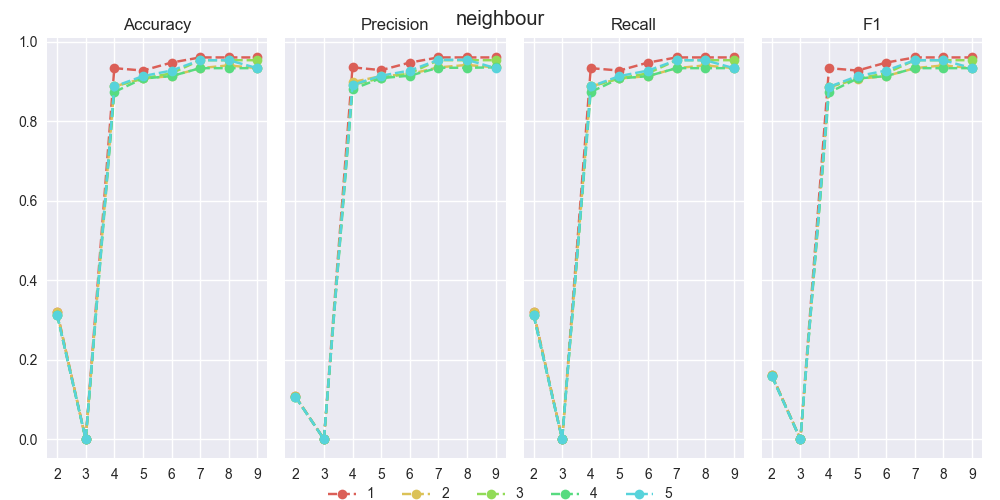
\includegraphics[width=\textwidth]{resources/plots/iris_KFold_neighbour.png}
        \caption{Wykres wartości miar dla zbioru "Iris" dla różnej liczby sąsiadów (kroswalidacja zwykła).}
    \end{figure}

    \begin{figure}[H]
        \center
        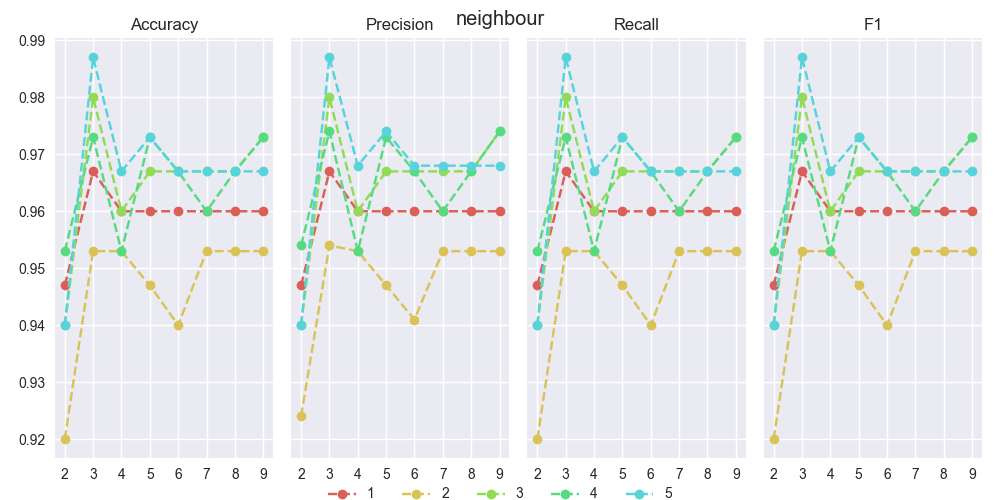
\includegraphics[width=\textwidth]{resources/plots/iris_StratifiedKFold_neighbour.png}
        \caption{Wykres wartości miar dla zbioru "Iris" dla różnej liczby sąsiadów (kroswalidacja stratyfikowana).}
    \end{figure}

    
\begin{table}[H]
    \begin{tabular}{c|c|cccccccc}
       \multirow{2}{*}{Wartość parametru} & \multirow{2}{*}{Metryka} & \multicolumn{8}{|c|}{Kroswalidacja} \\
         & & K = 2 & K = 3 & K = 4 & K = 5 & K = 6 & K = 7 & K = 8 & K = 9 \\ \hline
         1&Accuracy&0.32& 0.0& 0.933& 0.927& 0.947& 0.96& 0.96& 0.96\\ \hline
1&Precision&0.108& 0.0& 0.935& 0.928& 0.947& 0.96& 0.96& 0.96\\ \hline
1&Recall&0.32& 0.0& 0.933& 0.927& 0.947& 0.96& 0.96& 0.96\\ \hline
1&F1&0.162& 0.0& 0.933& 0.927& 0.947& 0.96& 0.96& 0.96\\ \hline
2&Accuracy&0.32& 0.0& 0.887& 0.907& 0.913& 0.933& 0.94& 0.933\\ \hline
2&Precision&0.108& 0.0& 0.898& 0.913& 0.918& 0.935& 0.941& 0.935\\ \hline
2&Recall&0.32& 0.0& 0.887& 0.907& 0.913& 0.933& 0.94& 0.933\\ \hline
2&F1&0.162& 0.0& 0.885& 0.906& 0.913& 0.933& 0.94& 0.933\\ \hline
3&Accuracy&0.313& 0.0& 0.887& 0.907& 0.92& 0.953& 0.953& 0.953\\ \hline
3&Precision&0.107& 0.0& 0.891& 0.908& 0.92& 0.953& 0.953& 0.953\\ \hline
3&Recall&0.313& 0.0& 0.887& 0.907& 0.92& 0.953& 0.953& 0.953\\ \hline
3&F1&0.159& 0.0& 0.886& 0.907& 0.92& 0.953& 0.953& 0.953\\ \hline
4&Accuracy&0.313& 0.0& 0.873& 0.907& 0.913& 0.933& 0.933& 0.933\\ \hline
4&Precision&0.107& 0.0& 0.88& 0.908& 0.914& 0.934& 0.934& 0.935\\ \hline
4&Recall&0.313& 0.0& 0.873& 0.907& 0.913& 0.933& 0.933& 0.933\\ \hline
4&F1&0.159& 0.0& 0.872& 0.907& 0.913& 0.933& 0.933& 0.933\\ \hline
5&Accuracy&0.313& 0.0& 0.887& 0.913& 0.927& 0.953& 0.953& 0.933\\ \hline
5&Precision&0.107& 0.0& 0.891& 0.914& 0.927& 0.954& 0.954& 0.933\\ \hline
5&Recall&0.313& 0.0& 0.887& 0.913& 0.927& 0.953& 0.953& 0.933\\ \hline
5&F1&0.159& 0.0& 0.886& 0.913& 0.927& 0.953& 0.953& 0.933 \\ \hline
    \end{tabular}
    \caption{Wartości miar dla zbioru "Iris" dla różnej liczby sąsiadów (kroswalidacja zwykła).}
\end{table}
    
    
\begin{table}[H]
    \begin{tabular}{c|c|cccccccc}
       \multirow{2}{*}{Wartość parametru} & \multirow{2}{*}{Metryka} & \multicolumn{8}{|c|}{Kroswalidacja} \\
         & & K = 2 & K = 3 & K = 4 & K = 5 & K = 6 & K = 7 & K = 8 & K = 9 \\ \hline
         1&Accuracy&0.947& 0.967& 0.96& 0.96& 0.96& 0.96& 0.96& 0.96\\ \hline
1&Precision&0.947& 0.967& 0.96& 0.96& 0.96& 0.96& 0.96& 0.96\\ \hline
1&Recall&0.947& 0.967& 0.96& 0.96& 0.96& 0.96& 0.96& 0.96\\ \hline
1&F1&0.947& 0.967& 0.96& 0.96& 0.96& 0.96& 0.96& 0.96\\ \hline
2&Accuracy&0.92& 0.953& 0.953& 0.947& 0.94& 0.953& 0.953& 0.953\\ \hline
2&Precision&0.924& 0.954& 0.953& 0.947& 0.941& 0.953& 0.953& 0.953\\ \hline
2&Recall&0.92& 0.953& 0.953& 0.947& 0.94& 0.953& 0.953& 0.953\\ \hline
2&F1&0.92& 0.953& 0.953& 0.947& 0.94& 0.953& 0.953& 0.953\\ \hline
3&Accuracy&0.94& 0.98& 0.96& 0.967& 0.967& 0.967& 0.967& 0.973\\ \hline
3&Precision&0.94& 0.98& 0.96& 0.967& 0.967& 0.967& 0.967& 0.974\\ \hline
3&Recall&0.94& 0.98& 0.96& 0.967& 0.967& 0.967& 0.967& 0.973\\ \hline
3&F1&0.94& 0.98& 0.96& 0.967& 0.967& 0.967& 0.967& 0.973\\ \hline
4&Accuracy&0.953& 0.973& 0.953& 0.973& 0.967& 0.96& 0.967& 0.973\\ \hline
4&Precision&0.954& 0.974& 0.953& 0.973& 0.967& 0.96& 0.967& 0.974\\ \hline
4&Recall&0.953& 0.973& 0.953& 0.973& 0.967& 0.96& 0.967& 0.973\\ \hline
4&F1&0.953& 0.973& 0.953& 0.973& 0.967& 0.96& 0.967& 0.973\\ \hline
5&Accuracy&0.94& 0.987& 0.967& 0.973& 0.967& 0.967& 0.967& 0.967\\ \hline
5&Precision&0.94& 0.987& 0.968& 0.974& 0.968& 0.968& 0.968& 0.968\\ \hline
5&Recall&0.94& 0.987& 0.967& 0.973& 0.967& 0.967& 0.967& 0.967\\ \hline
5&F1&0.94& 0.987& 0.967& 0.973& 0.967& 0.967& 0.967& 0.967 \\ \hline
    \end{tabular}
    \caption{Wartości miar dla zbioru "Iris" dla różnej liczby sąsiadów (kroswalidacja stratyfikowana).}
\end{table}
    

    \pagebreak

    \begin{figure}[H]
        \center
        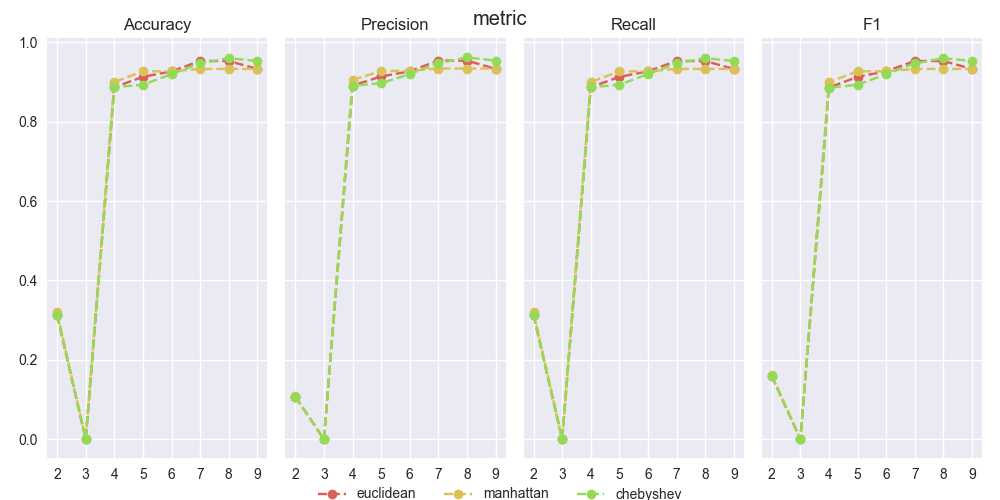
\includegraphics[width=\textwidth]{resources/plots/iris_KFold_metric.png}
        \caption{Wykres wartości miar dla zbioru "Iris" dla różnych metryk odległości (kroswalidacja zwykła).}
    \end{figure}

    \begin{figure}[H]
        \center
        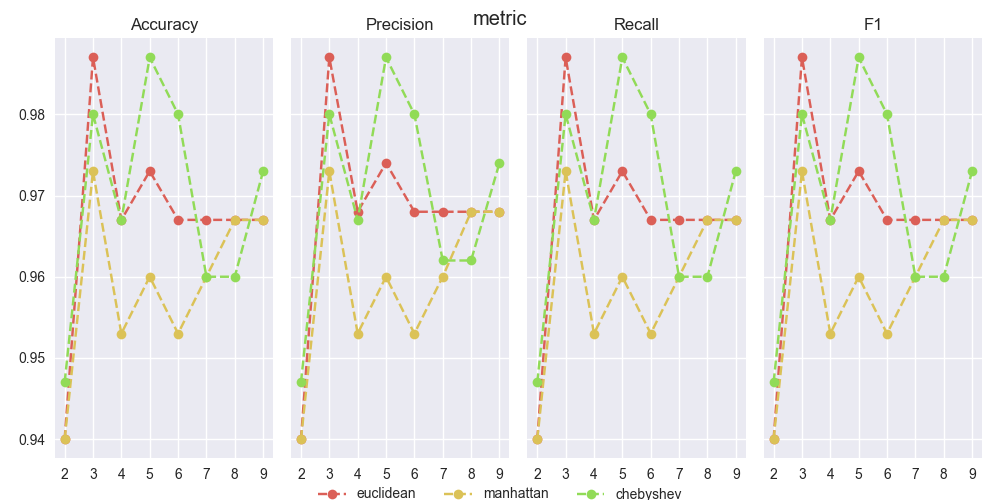
\includegraphics[width=\textwidth]{resources/plots/iris_StratifiedKFold_metric.png}
        \caption{Wykres wartości miar dla zbioru "Iris" dla różnych metryk odległości (kroswalidacja stratyfikowana).}
    \end{figure}

    
\begin{table}[H]
    \begin{tabular}{c|c|cccccccc}
       \multirow{2}{*}{Wartość parametru} & \multirow{2}{*}{Metryka} & \multicolumn{8}{|c|}{Kroswalidacja} \\
         & & K = 2 & K = 3 & K = 4 & K = 5 & K = 6 & K = 7 & K = 8 & K = 9 \\ \hline
         euclidean&Accuracy&0.313& 0.0& 0.887& 0.913& 0.927& 0.953& 0.953& 0.933\\ \hline
euclidean&Precision&0.107& 0.0& 0.891& 0.914& 0.927& 0.954& 0.954& 0.933\\ \hline
euclidean&Recall&0.313& 0.0& 0.887& 0.913& 0.927& 0.953& 0.953& 0.933\\ \hline
euclidean&F1&0.159& 0.0& 0.886& 0.913& 0.927& 0.953& 0.953& 0.933\\ \hline
manhattan&Accuracy&0.32& 0.0& 0.9& 0.927& 0.927& 0.933& 0.933& 0.933\\ \hline
manhattan&Precision&0.108& 0.0& 0.905& 0.928& 0.928& 0.934& 0.934& 0.934\\ \hline
manhattan&Recall&0.32& 0.0& 0.9& 0.927& 0.927& 0.933& 0.933& 0.933\\ \hline
manhattan&F1&0.162& 0.0& 0.9& 0.927& 0.927& 0.933& 0.933& 0.933\\ \hline
chebyshev&Accuracy&0.313& 0.0& 0.887& 0.893& 0.92& 0.947& 0.96& 0.953\\ \hline
chebyshev&Precision&0.107& 0.0& 0.891& 0.897& 0.92& 0.947& 0.962& 0.954\\ \hline
chebyshev&Recall&0.313& 0.0& 0.887& 0.893& 0.92& 0.947& 0.96& 0.953\\ \hline
chebyshev&F1&0.159& 0.0& 0.886& 0.893& 0.92& 0.947& 0.96& 0.953 \\ \hline
    \end{tabular}
    \caption{Wartości miar dla zbioru "Iris" dla różnych metryk odległości (kroswalidacja zwykła).}
\end{table}
    
    
\begin{table}[H]
    \begin{tabular}{c|c|cccccccc}
       \multirow{2}{*}{Wartość parametru} & \multirow{2}{*}{Metryka} & \multicolumn{8}{|c|}{Kroswalidacja} \\
         & & K = 2 & K = 3 & K = 4 & K = 5 & K = 6 & K = 7 & K = 8 & K = 9 \\ \hline
         euclidean&Accuracy&0.94& 0.987& 0.967& 0.973& 0.967& 0.967& 0.967& 0.967\\ \hline
euclidean&Precision&0.94& 0.987& 0.968& 0.974& 0.968& 0.968& 0.968& 0.968\\ \hline
euclidean&Recall&0.94& 0.987& 0.967& 0.973& 0.967& 0.967& 0.967& 0.967\\ \hline
euclidean&F1&0.94& 0.987& 0.967& 0.973& 0.967& 0.967& 0.967& 0.967\\ \hline
manhattan&Accuracy&0.94& 0.973& 0.953& 0.96& 0.953& 0.96& 0.967& 0.967\\ \hline
manhattan&Precision&0.94& 0.973& 0.953& 0.96& 0.953& 0.96& 0.968& 0.968\\ \hline
manhattan&Recall&0.94& 0.973& 0.953& 0.96& 0.953& 0.96& 0.967& 0.967\\ \hline
manhattan&F1&0.94& 0.973& 0.953& 0.96& 0.953& 0.96& 0.967& 0.967\\ \hline
chebyshev&Accuracy&0.947& 0.98& 0.967& 0.987& 0.98& 0.96& 0.96& 0.973\\ \hline
chebyshev&Precision&0.947& 0.98& 0.967& 0.987& 0.98& 0.962& 0.962& 0.974\\ \hline
chebyshev&Recall&0.947& 0.98& 0.967& 0.987& 0.98& 0.96& 0.96& 0.973\\ \hline
chebyshev&F1&0.947& 0.98& 0.967& 0.987& 0.98& 0.96& 0.96& 0.973 \\ \hline
    \end{tabular}
    \caption{Wartości miar dla zbioru "Iris" dla różnych metryk odległości (kroswalidacja stratyfikowana).}
\end{table}
    

    \pagebreak

    \begin{figure}[H]
        \center
        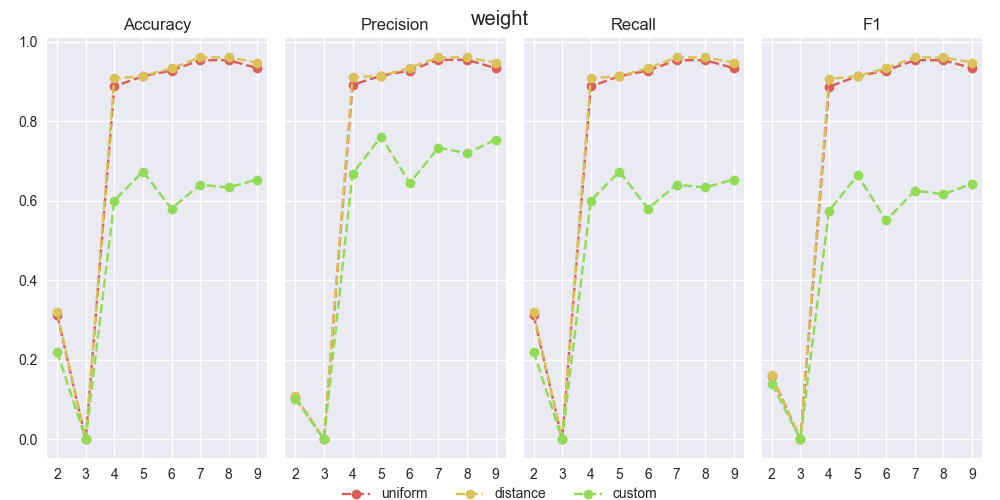
\includegraphics[width=\textwidth]{resources/plots/iris_KFold_weight.png}
        \caption{Wykres wartości miar dla zbioru "Iris" dla różnych sposobów głosowania (kroswalidacja zwykła).}
    \end{figure}

    \begin{figure}[H]
        \center
        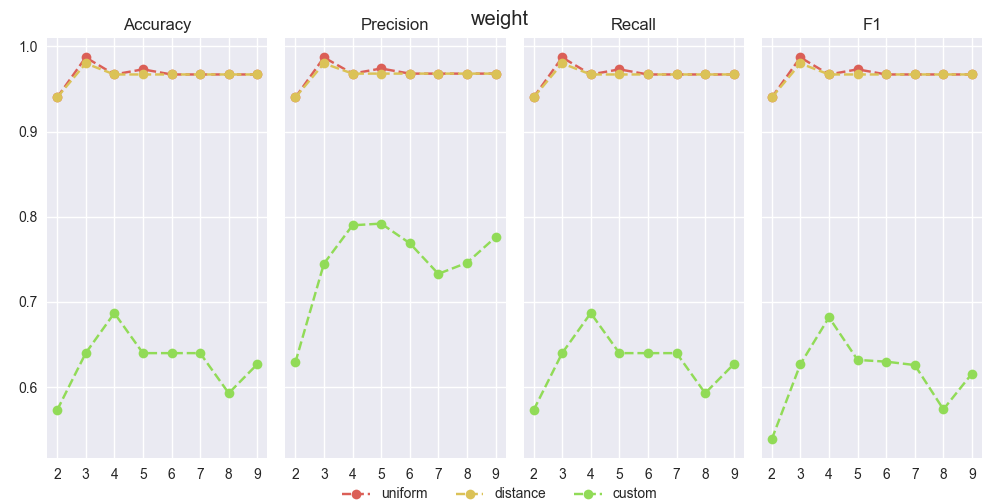
\includegraphics[width=\textwidth]{resources/plots/iris_StratifiedKFold_weight.png}
        \caption{Wykres wartości miar dla zbioru "Iris" dla różnych sposobów głosowania (kroswalidacja stratyfikowana).}
    \end{figure}

    
\begin{table}[H]
    \begin{tabular}{c|c|cccccccc}
       \multirow{2}{*}{Wartość parametru} & \multirow{2}{*}{Metryka} & \multicolumn{8}{|c|}{Kroswalidacja} \\
         & & K = 2 & K = 3 & K = 4 & K = 5 & K = 6 & K = 7 & K = 8 & K = 9 \\ \hline
         uniform&Accuracy&0.313& 0.0& 0.887& 0.913& 0.927& 0.953& 0.953& 0.933\\ \hline
uniform&Precision&0.107& 0.0& 0.891& 0.914& 0.927& 0.954& 0.954& 0.933\\ \hline
uniform&Recall&0.313& 0.0& 0.887& 0.913& 0.927& 0.953& 0.953& 0.933\\ \hline
uniform&F1&0.159& 0.0& 0.886& 0.913& 0.927& 0.953& 0.953& 0.933\\ \hline
distance&Accuracy&0.32& 0.0& 0.907& 0.913& 0.933& 0.96& 0.96& 0.947\\ \hline
distance&Precision&0.108& 0.0& 0.91& 0.914& 0.934& 0.96& 0.96& 0.947\\ \hline
distance&Recall&0.32& 0.0& 0.907& 0.913& 0.933& 0.96& 0.96& 0.947\\ \hline
distance&F1&0.162& 0.0& 0.906& 0.913& 0.933& 0.96& 0.96& 0.947\\ \hline
custom&Accuracy&0.233& 0.0& 0.607& 0.567& 0.613& 0.593& 0.673& 0.627\\ \hline
custom&Precision&0.112& 0.0& 0.681& 0.691& 0.699& 0.729& 0.803& 0.726\\ \hline
custom&Recall&0.233& 0.0& 0.607& 0.567& 0.613& 0.593& 0.673& 0.627\\ \hline
custom&F1&0.152& 0.0& 0.583& 0.535& 0.591& 0.573& 0.67& 0.61 \\ \hline
    \end{tabular}
    \caption{Wartości miar dla zbioru "Iris" dla różnych sposobów głosowania (kroswalidacja zwykła).}
\end{table}
    
    
\begin{table}[H]
    \begin{tabular}{c|c|cccccccc}
       \multirow{2}{*}{Wartość parametru} & \multirow{2}{*}{Metryka} & \multicolumn{8}{|c|}{Kroswalidacja} \\
         & & K = 2 & K = 3 & K = 4 & K = 5 & K = 6 & K = 7 & K = 8 & K = 9 \\ \hline
         uniform&Accuracy&0.94& 0.987& 0.967& 0.973& 0.967& 0.967& 0.967& 0.967\\ \hline
uniform&Precision&0.94& 0.987& 0.968& 0.974& 0.968& 0.968& 0.968& 0.968\\ \hline
uniform&Recall&0.94& 0.987& 0.967& 0.973& 0.967& 0.967& 0.967& 0.967\\ \hline
uniform&F1&0.94& 0.987& 0.967& 0.973& 0.967& 0.967& 0.967& 0.967\\ \hline
distance&Accuracy&0.94& 0.98& 0.967& 0.967& 0.967& 0.967& 0.967& 0.967\\ \hline
distance&Precision&0.94& 0.98& 0.968& 0.968& 0.968& 0.968& 0.968& 0.968\\ \hline
distance&Recall&0.94& 0.98& 0.967& 0.967& 0.967& 0.967& 0.967& 0.967\\ \hline
distance&F1&0.94& 0.98& 0.967& 0.967& 0.967& 0.967& 0.967& 0.967\\ \hline
custom&Accuracy&0.653& 0.573& 0.687& 0.647& 0.62& 0.68& 0.7& 0.673\\ \hline
custom&Precision&0.769& 0.665& 0.778& 0.752& 0.75& 0.764& 0.795& 0.786\\ \hline
custom&Recall&0.653& 0.573& 0.687& 0.647& 0.62& 0.68& 0.7& 0.673\\ \hline
custom&F1&0.644& 0.544& 0.675& 0.634& 0.605& 0.67& 0.692& 0.668 \\ \hline
    \end{tabular}
    \caption{Wartości miar dla zbioru "Iris" dla różnych sposobów głosowania (kroswalidacja stratyfikowana).}
\end{table}
    
    \section{Zbiór Diabetes}
\subsection{Algorytm Adaboost}

\begin{tabular}{llrrrrrrrr}
\hline
          & \{\} & \multicolumn{8}{l}{Miara F1} \\
          & Liczba foldów &        2 &      3 &      4 &      5 &      6 &      7 &      8 &      9 \\
Parametr & Wartość parametru &          &        &        &        &        &        &        &        \\
\hline
algorithm & SAMME &    0.589 &  0.598 &  0.614 &  0.574 &  0.603 &  0.588 &  0.602 &  0.570 \\
          & SAMME.R &    0.551 &  0.597 &  0.612 &  0.589 &  0.583 &  0.596 &  0.599 &  0.611 \\
\hline
\end{tabular}

\begin{figure}[H]
    \center
    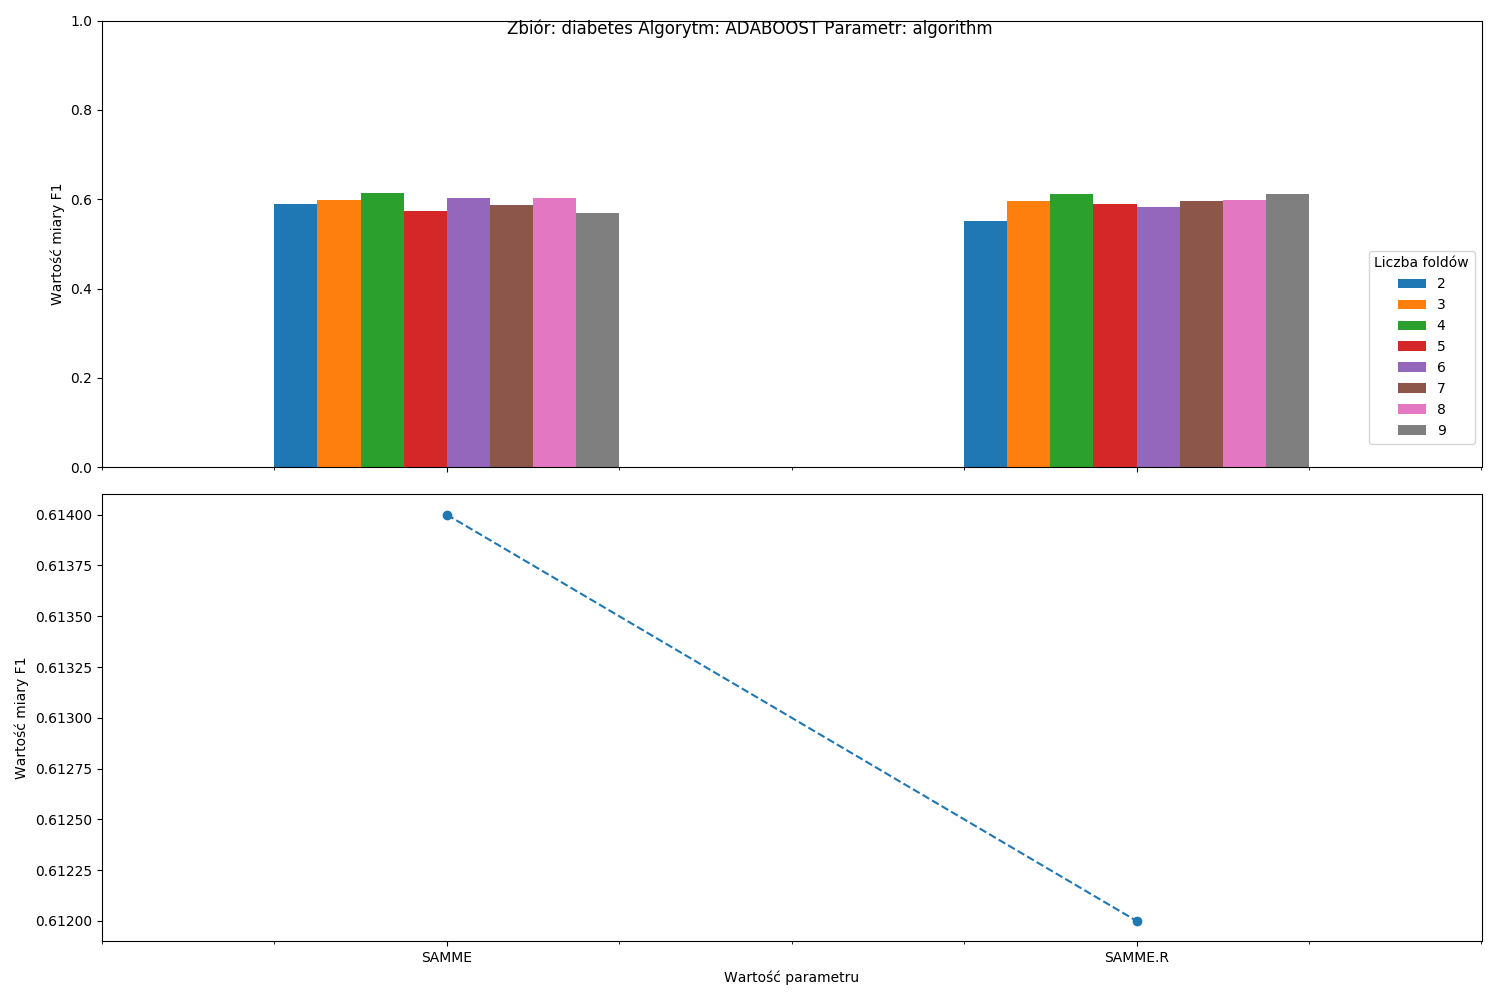
\includegraphics[width=\textwidth]{resources/plots/diabetes_adaboost_algorithm.png}
    \caption{Wykres wartości miary F1 dla zbioru "Diabetes" algorytmu "Adaboost" przy ustalonym parametrze "algorithm".}   
\end{figure}

\pagebreak
                    
\begin{tabular}{llrrrrrrrr}
\hline
              & \{\} & \multicolumn{8}{l}{Miara F1} \\
              & Liczba foldów &        2 &      3 &      4 &      5 &      6 &      7 &      8 &      9 \\
Parametr & Wartość parametru &          &        &        &        &        &        &        &        \\
\hline
learning\_rate & 0.0001 &    0.565 &  0.591 &  0.603 &  0.598 &  0.583 &  0.631 &  0.617 &  0.600 \\
              & 0.001 &    0.625 &  0.593 &  0.614 &  0.588 &  0.596 &  0.612 &  0.602 &  0.597 \\
              & 0.01 &    0.589 &  0.598 &  0.593 &  0.588 &  0.579 &  0.577 &  0.602 &  0.572 \\
              & 0.1 &    0.585 &  0.586 &  0.604 &  0.581 &  0.588 &  0.609 &  0.602 &  0.616 \\
\hline
\end{tabular}

\begin{figure}[H]
    \center
    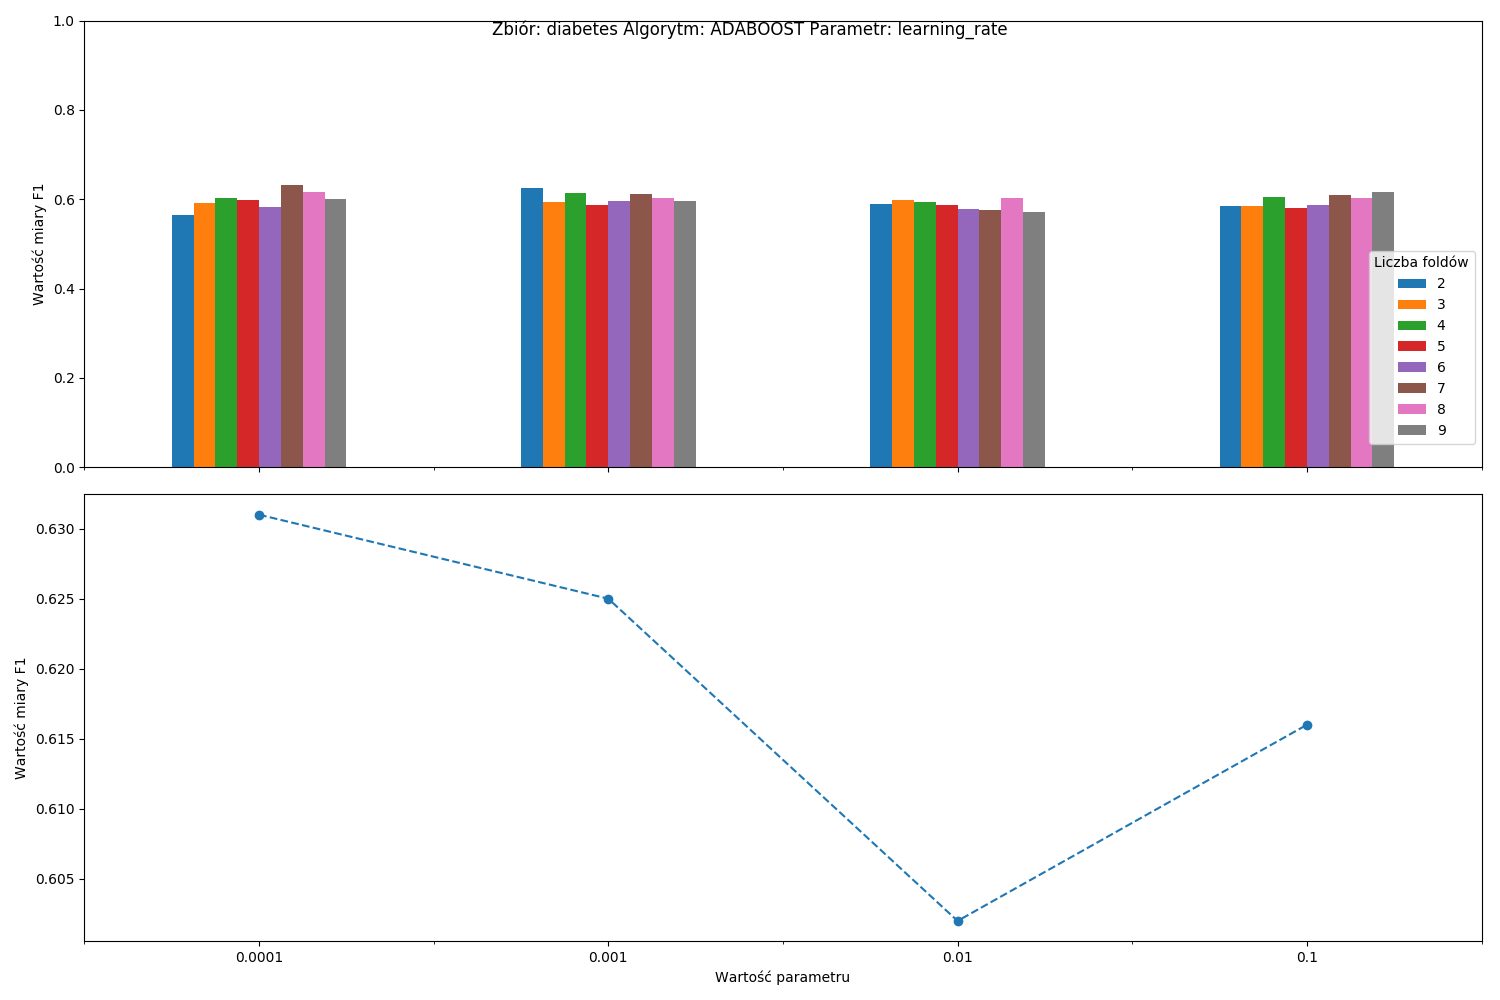
\includegraphics[width=\textwidth]{resources/plots/diabetes_adaboost_learning_rate.png}
    \caption{Wykres wartości miary F1 dla zbioru "Diabetes" algorytmu "Adaboost" przy ustalonym parametrze "learning\_rate".}
\end{figure}

\pagebreak
                    
\begin{tabular}{llrrrrrrrr}
\hline
             & \{\} & \multicolumn{8}{l}{Miara F1} \\
             & Liczba foldów &        2 &      3 &      4 &      5 &      6 &      7 &      8 &      9 \\
Parametr & Wartość parametru &          &        &        &        &        &        &        &        \\
\hline
n\_estimators & 10.0 &    0.574 &  0.587 &  0.590 &  0.593 &  0.615 &  0.617 &  0.607 &  0.586 \\
             & 25.0 &    0.567 &  0.597 &  0.563 &  0.563 &  0.566 &  0.590 &  0.584 &  0.587 \\
             & 50.0 &    0.568 &  0.576 &  0.585 &  0.602 &  0.612 &  0.605 &  0.635 &  0.579 \\
             & 75.0 &    0.576 &  0.591 &  0.609 &  0.590 &  0.585 &  0.595 &  0.597 &  0.618 \\
             & 99.0 &    0.592 &  0.576 &  0.600 &  0.577 &  0.595 &  0.594 &  0.588 &  0.622 \\
\hline
\end{tabular}

\begin{figure}[H]
    \center
    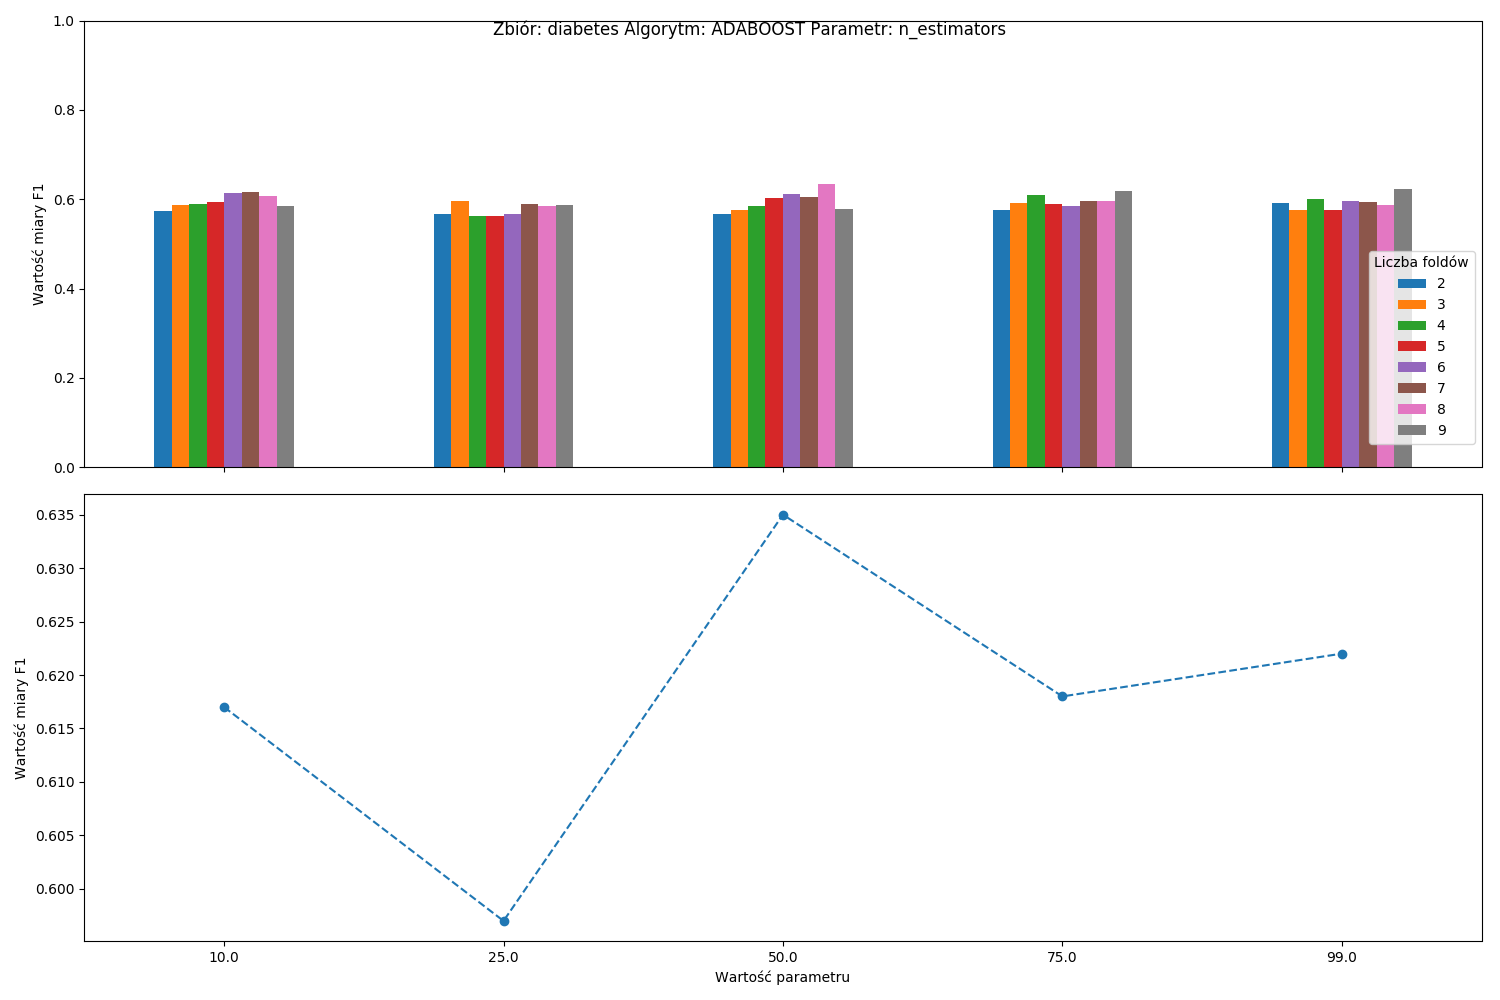
\includegraphics[width=\textwidth]{resources/plots/diabetes_adaboost_n_estimators.png}
    \caption{Wykres wartości miary F1 dla zbioru "Diabetes" algorytmu "Adaboost" przy ustalonym parametrze "n\_estimators".}
\end{figure}

\pagebreak
                    
\subsection{Algorytm Bagging}

\begin{tabular}{llrrrrrrrr}
\hline
          & \{\} & \multicolumn{8}{l}{Miara F1} \\
          & Liczba foldów &        2 &      3 &      4 &      5 &      6 &     7 &      8 &      9 \\
Parametr & Wartość parametru &          &        &        &        &        &       &        &        \\
\hline
bootstrap & False &    0.563 &  0.579 &  0.586 &  0.573 &  0.580 &  0.61 &  0.614 &  0.588 \\
          & True &    0.603 &  0.610 &  0.598 &  0.612 &  0.601 &  0.59 &  0.597 &  0.578 \\
\hline
\end{tabular}

\begin{figure}[H]
    \center
    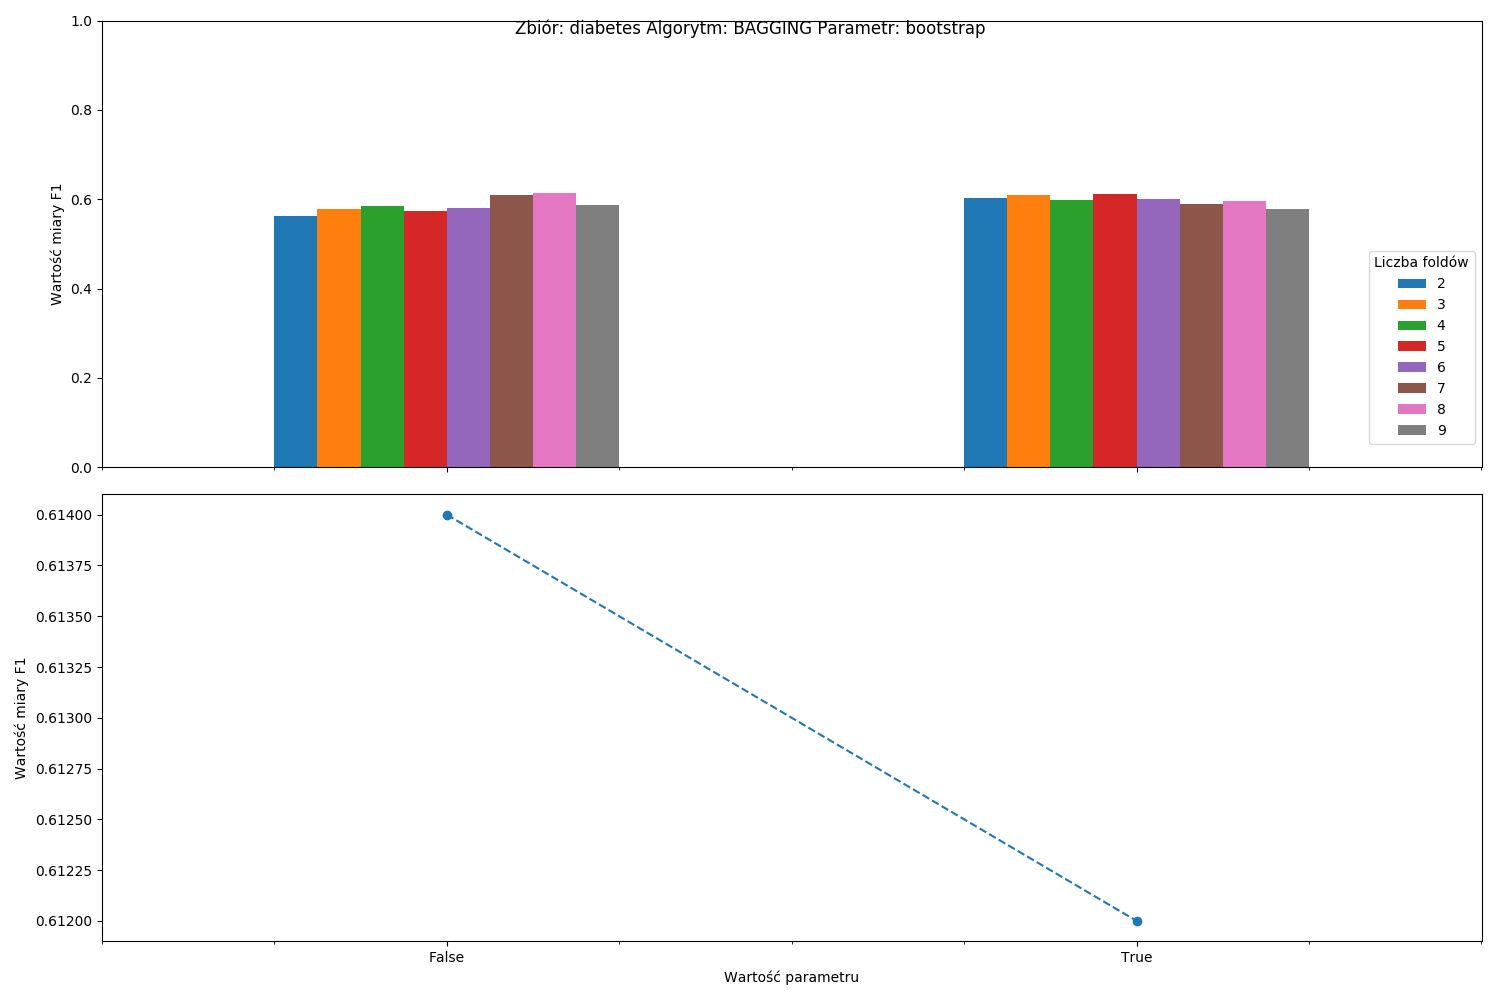
\includegraphics[width=\textwidth]{resources/plots/diabetes_bagging_bootstrap.png}
    \caption{Wykres wartości miary F1 dla zbioru "Diabetes" algorytmu "Bagging" przy ustalonym parametrze "bootstrap".}   
\end{figure}

\pagebreak
                    
\begin{tabular}{llrrrrrrrr}
\hline
            & \{\} & \multicolumn{8}{l}{Miara F1} \\
            & Liczba foldów &        2 &      3 &      4 &      5 &      6 &      7 &      8 &      9 \\
Parametr & Wartość parametru &          &        &        &        &        &        &        &        \\
\hline
max\_samples & 0.25 &    0.567 &  0.556 &  0.627 &  0.575 &  0.596 &  0.619 &  0.617 &  0.603 \\
            & 0.5 &    0.574 &  0.594 &  0.636 &  0.592 &  0.572 &  0.597 &  0.615 &  0.598 \\
            & 0.75 &    0.576 &  0.566 &  0.626 &  0.580 &  0.628 &  0.598 &  0.608 &  0.604 \\
            & 1.0 &    0.559 &  0.596 &  0.589 &  0.604 &  0.573 &  0.595 &  0.599 &  0.591 \\
\hline
\end{tabular}

\begin{figure}[H]
    \center
    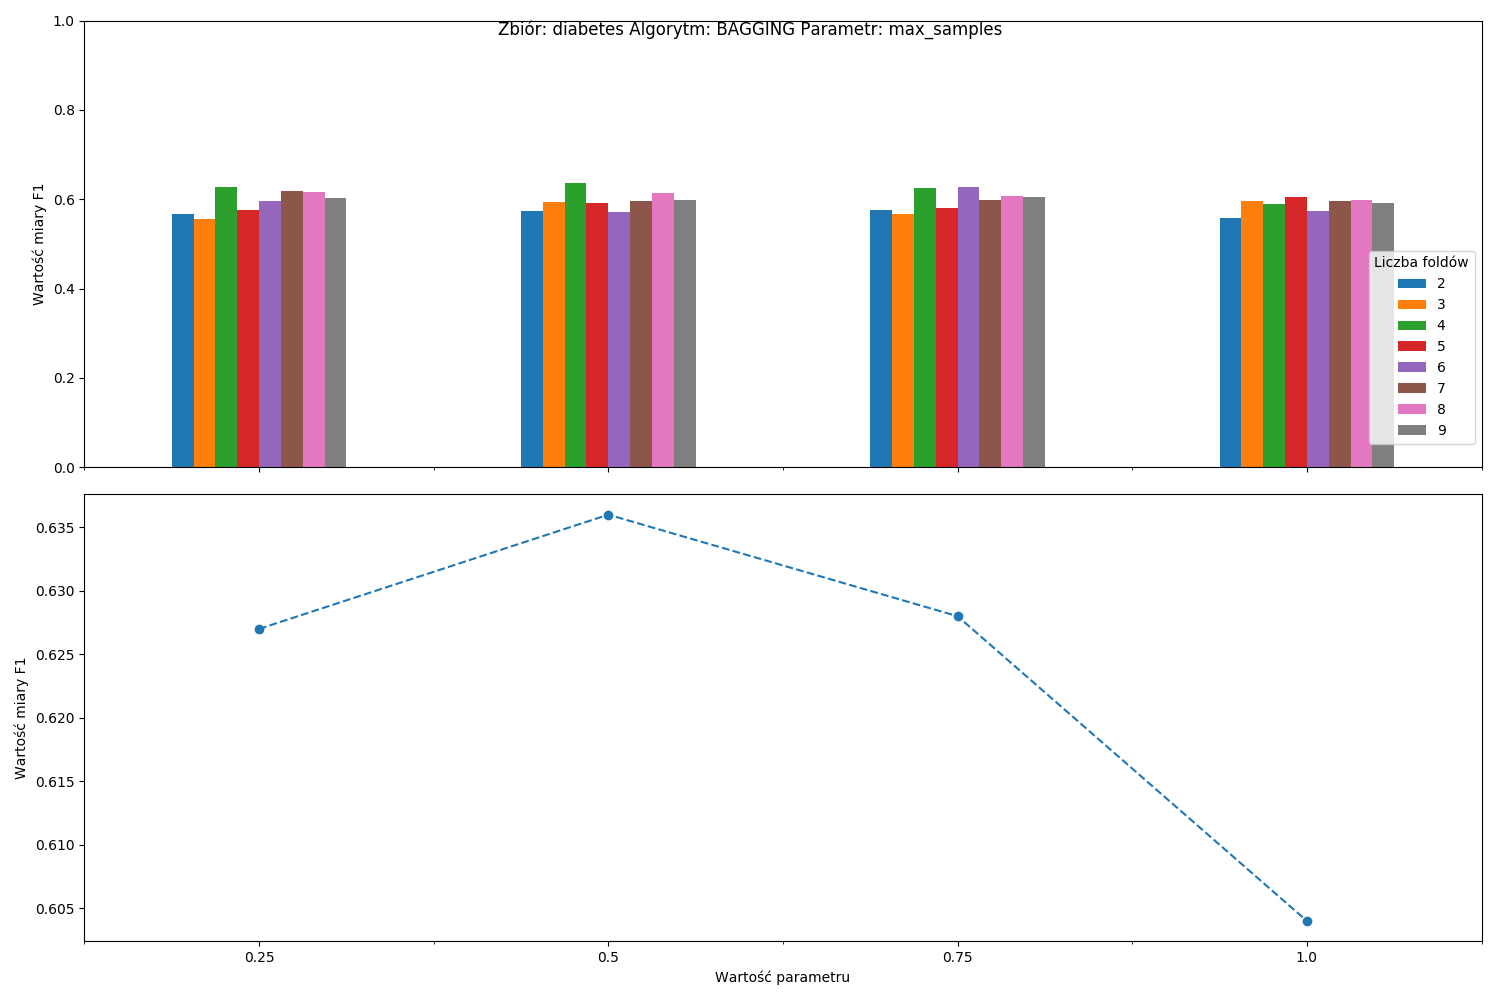
\includegraphics[width=\textwidth]{resources/plots/diabetes_bagging_max_samples.png}
    \caption{Wykres wartości miary F1 dla zbioru "Diabetes" algorytmu "Bagging" przy ustalonym parametrze "max\_samples".}
\end{figure}

\pagebreak
                    
\begin{tabular}{llrrrrrrrr}
\hline
             & \{\} & \multicolumn{8}{l}{Miara F1} \\
             & Liczba foldów &        2 &      3 &      4 &      5 &      6 &      7 &      8 &      9 \\
Parametr & Wartość parametru &          &        &        &        &        &        &        &        \\
\hline
n\_estimators & 10 &    0.566 &  0.606 &  0.601 &  0.557 &  0.585 &  0.595 &  0.594 &  0.598 \\
             & 25 &    0.575 &  0.591 &  0.580 &  0.578 &  0.606 &  0.616 &  0.595 &  0.575 \\
             & 50 &    0.568 &  0.567 &  0.578 &  0.603 &  0.581 &  0.587 &  0.590 &  0.577 \\
             & 75 &    0.531 &  0.597 &  0.600 &  0.581 &  0.602 &  0.584 &  0.589 &  0.599 \\
             & 99 &    0.542 &  0.616 &  0.623 &  0.575 &  0.615 &  0.600 &  0.592 &  0.573 \\
\hline
\end{tabular}

\begin{figure}[H]
    \center
    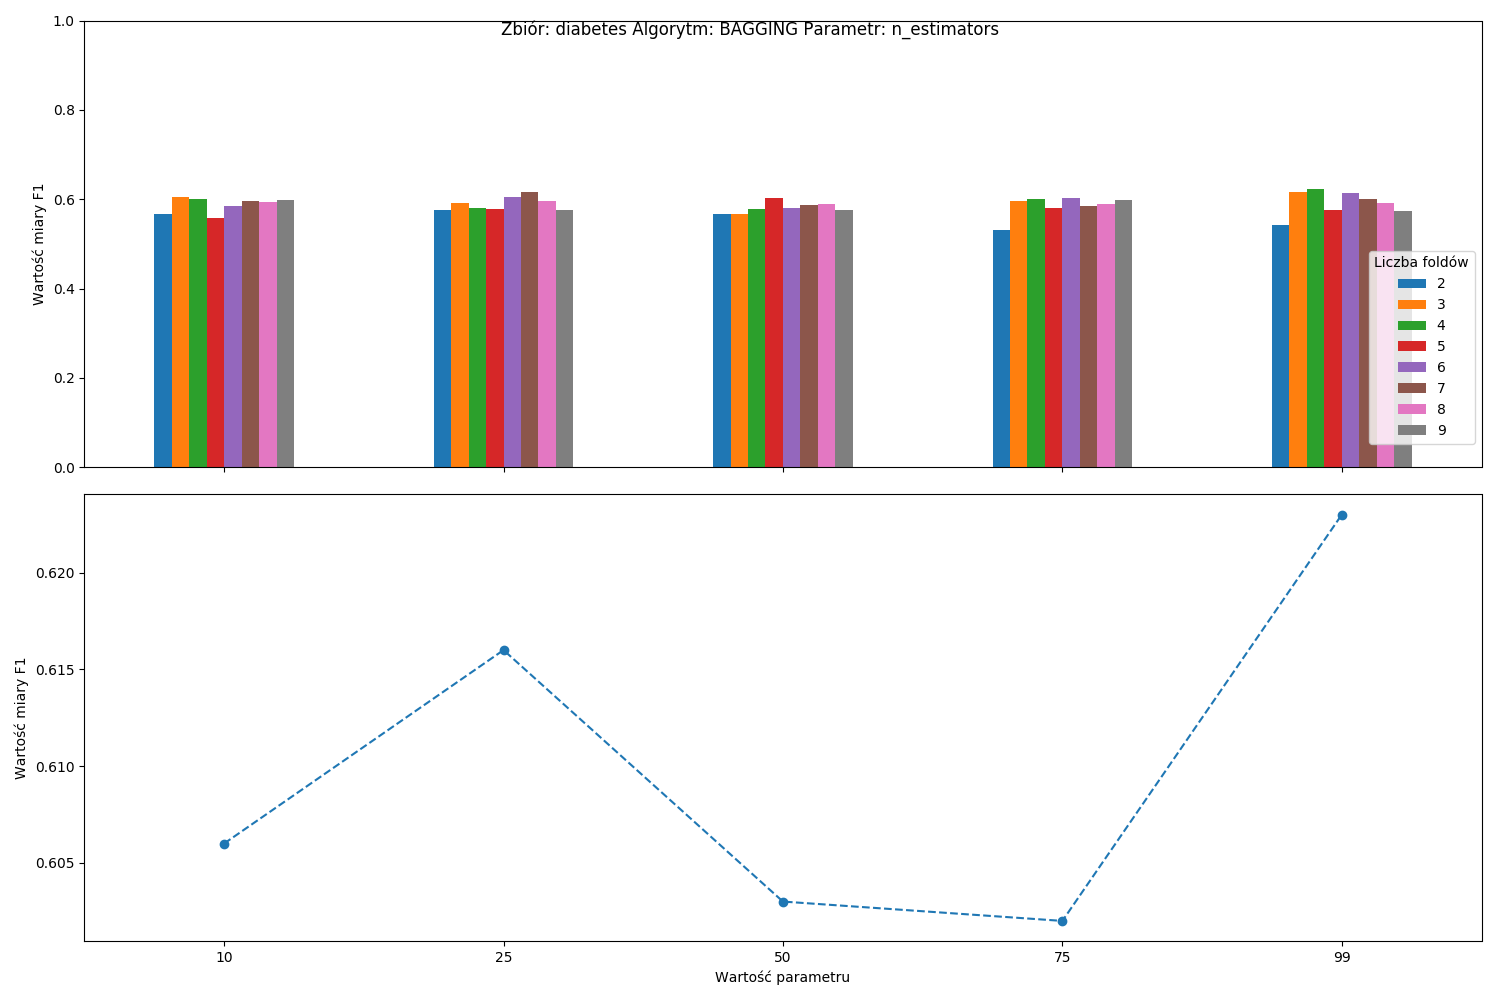
\includegraphics[width=\textwidth]{resources/plots/diabetes_bagging_n_estimators.png}
    \caption{Wykres wartości miary F1 dla zbioru "Diabetes" algorytmu "Bagging" przy ustalonym parametrze "n\_estimators".}
\end{figure}

\pagebreak
                    
\subsection{Algorytm Random-forest}

\begin{tabular}{llrrrrrrrr}
\hline
          & \{\} & \multicolumn{8}{l}{Miara F1} \\
          & Liczba foldów &        2 &      3 &      4 &      5 &      6 &      7 &      8 &      9 \\
Parametr & Wartość parametru &          &        &        &        &        &        &        &        \\
\hline
bootstrap & False &    0.593 &  0.593 &  0.600 &  0.593 &  0.573 &  0.625 &  0.612 &  0.591 \\
          & True &    0.591 &  0.612 &  0.627 &  0.596 &  0.626 &  0.583 &  0.589 &  0.592 \\
\hline
\end{tabular}

\begin{figure}[H]
    \center
    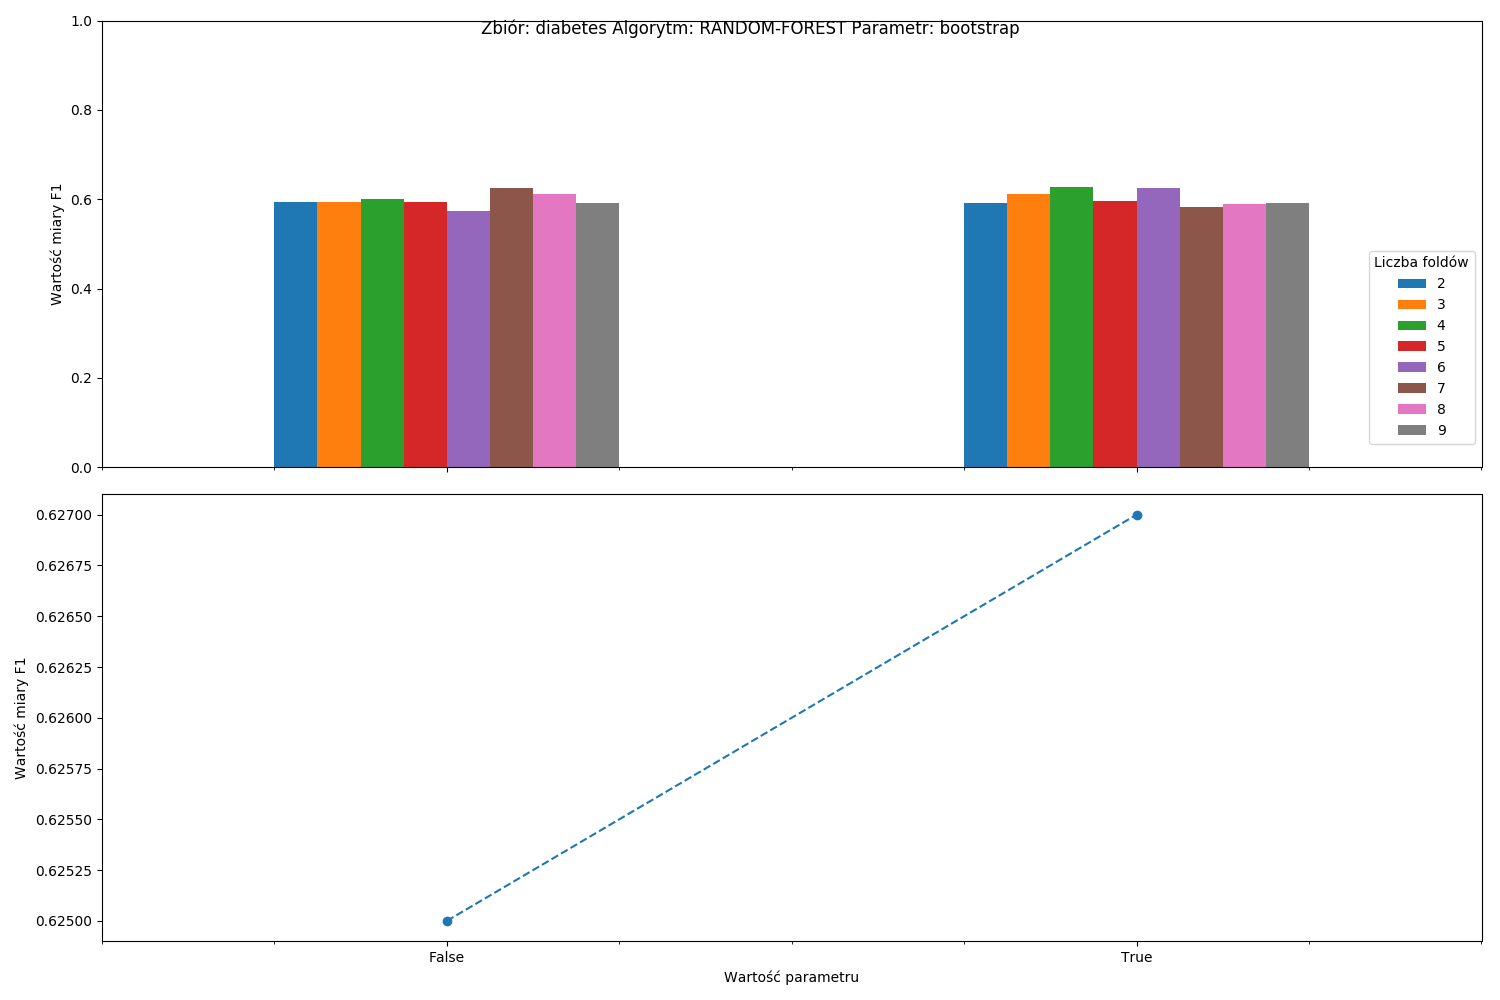
\includegraphics[width=\textwidth]{resources/plots/diabetes_random-forest_bootstrap.png}
    \caption{Wykres wartości miary F1 dla zbioru "Diabetes" algorytmu "Random-forest" przy ustalonym parametrze "bootstrap".}   
\end{figure}                    

\pagebreak

\begin{tabular}{llrrrrrrrr}
\hline
          & \{\} & \multicolumn{8}{l}{Miara F1} \\
          & Liczba foldów &        2 &      3 &      4 &      5 &      6 &      7 &      8 &      9 \\
Parametr & Wartość parametru &          &        &        &        &        &        &        &        \\
\hline
criterion & entropy &    0.577 &  0.590 &  0.610 &  0.589 &  0.592 &  0.615 &  0.577 &  0.595 \\
          & gini &    0.551 &  0.597 &  0.606 &  0.567 &  0.604 &  0.619 &  0.589 &  0.575 \\
\hline
\end{tabular}

\begin{figure}[H]
    \center
    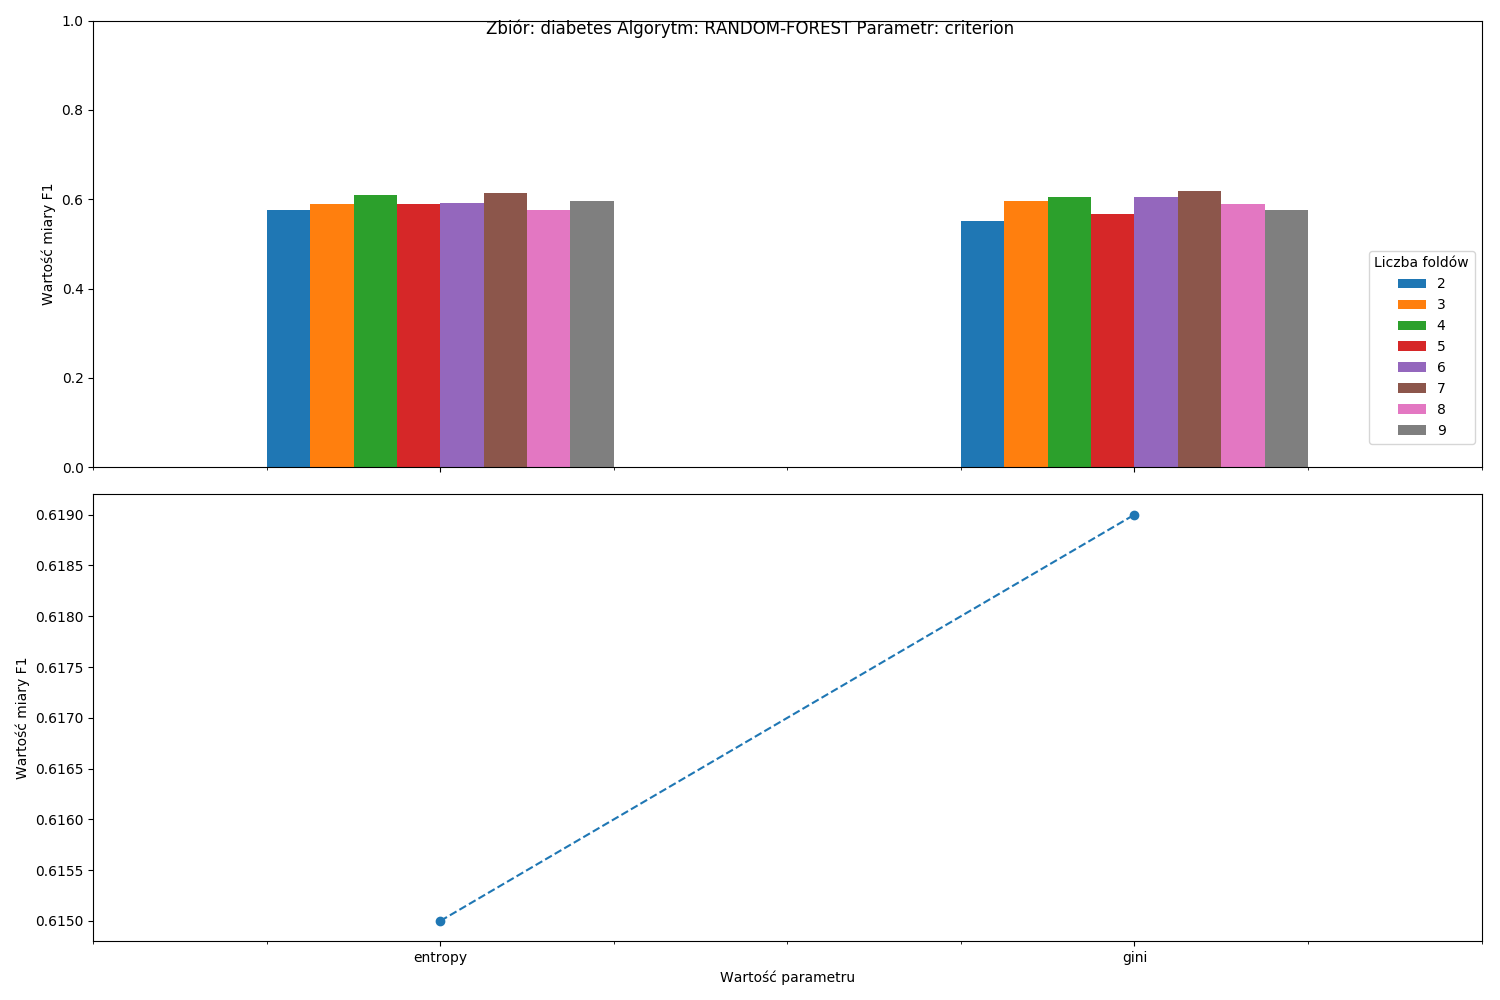
\includegraphics[width=\textwidth]{resources/plots/diabetes_random-forest_criterion.png}
    \caption{Wykres wartości miary F1 dla zbioru "Diabetes" algorytmu "Random-forest" przy ustalonym parametrze "criterion".}   
\end{figure}                    

\pagebreak

\begin{tabular}{llrrrrrrrr}
\hline
             & \{\} & \multicolumn{8}{l}{Miara F1} \\
             & Liczba foldów &        2 &      3 &      4 &      5 &      6 &      7 &      8 &      9 \\
Parametr & Wartość parametru &          &        &        &        &        &        &        &        \\
\hline
n\_estimators & 10 &    0.579 &  0.585 &  0.581 &  0.574 &  0.577 &  0.639 &  0.608 &  0.615 \\
             & 25 &    0.571 &  0.554 &  0.581 &  0.567 &  0.588 &  0.617 &  0.580 &  0.616 \\
             & 50 &    0.587 &  0.583 &  0.589 &  0.575 &  0.583 &  0.593 &  0.597 &  0.607 \\
             & 75 &    0.568 &  0.576 &  0.604 &  0.578 &  0.623 &  0.574 &  0.589 &  0.587 \\
             & 99 &    0.598 &  0.581 &  0.598 &  0.580 &  0.602 &  0.586 &  0.600 &  0.597 \\
\hline
\end{tabular}

\begin{figure}[H]
    \center
    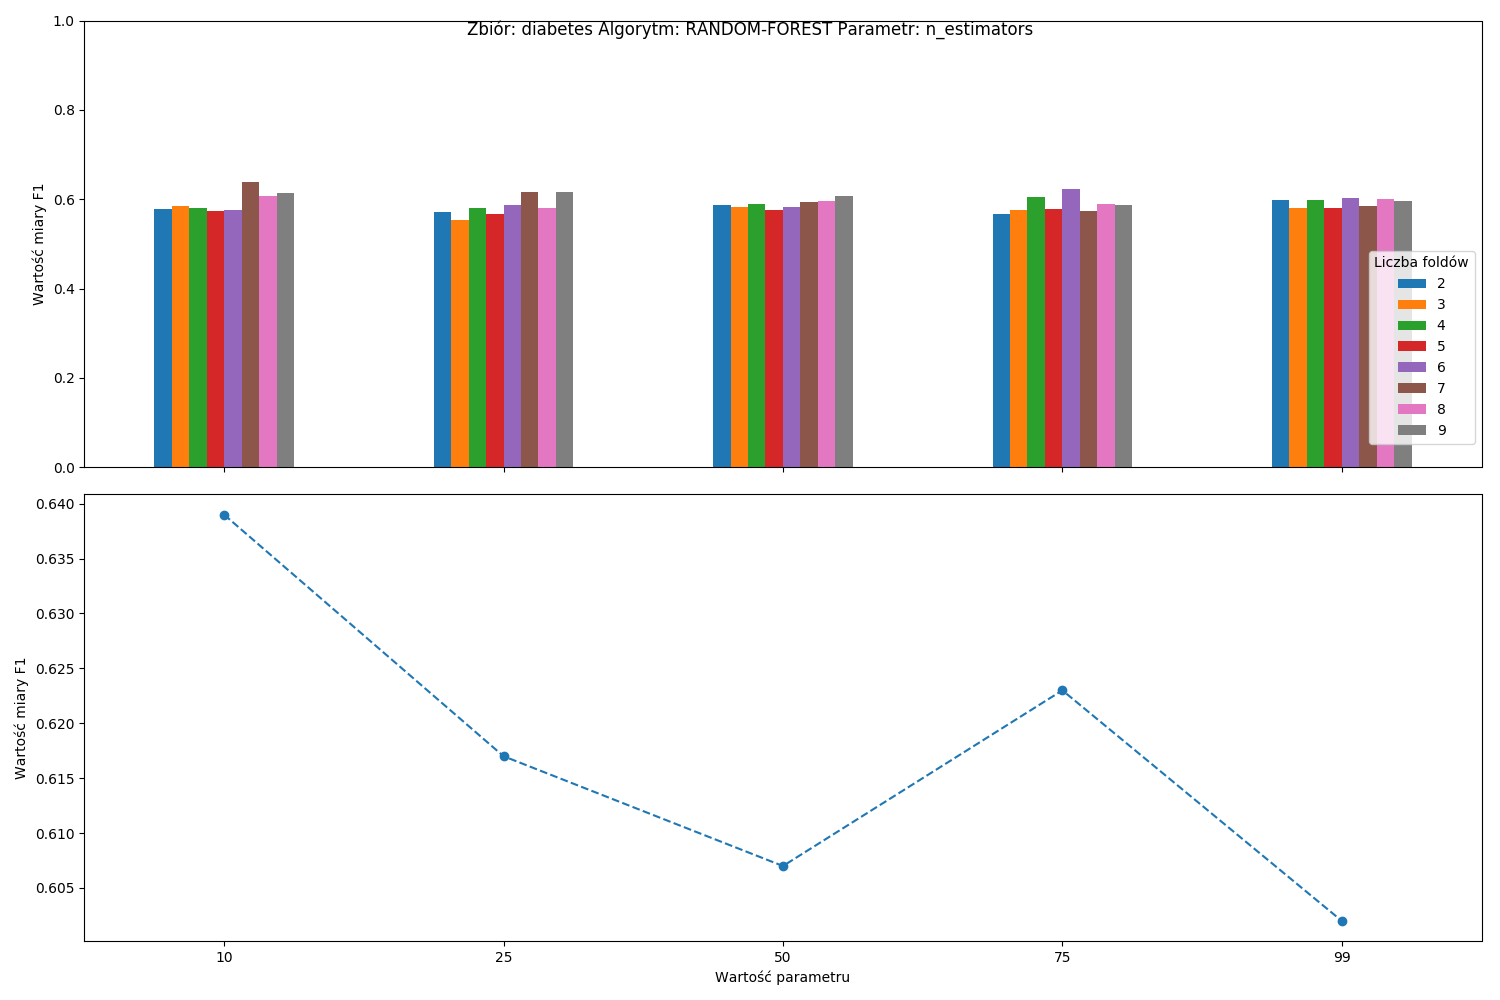
\includegraphics[width=\textwidth]{resources/plots/diabetes_random-forest_n_estimators.png}
    \caption{Wykres wartości miary F1 dla zbioru "Diabetes" algorytmu "Random-forest" przy ustalonym parametrze "n\_estimators".}
\end{figure}                    
                    
\pagebreak


\begin{tabular}{llrrrrrrrr}
\hline
             & \{\} & \multicolumn{8}{l}{Miara F1} \\
             & Liczba foldów &        2 &      3 &      4 &      5 &      6 &      7 &      8 &      9 \\
Parametr & Wartość parametru &          &        &        &        &        &        &        &        \\
\hline
max\_features & 0.25 &    0.563 &  0.596 &  0.568 &  0.578 &  0.601 &  0.595 &  0.612 &  0.605 \\
             & 0.5 &    0.580 &  0.604 &  0.606 &  0.591 &  0.577 &  0.588 &  0.594 &  0.590 \\
             & 0.75 &    0.572 &  0.613 &  0.585 &  0.576 &  0.601 &  0.587 &  0.611 &  0.606 \\
             & 1.0 &    0.561 &  0.580 &  0.610 &  0.563 &  0.572 &  0.633 &  0.598 &  0.607 \\
\hline
\end{tabular}

\begin{figure}[H]
    \center
    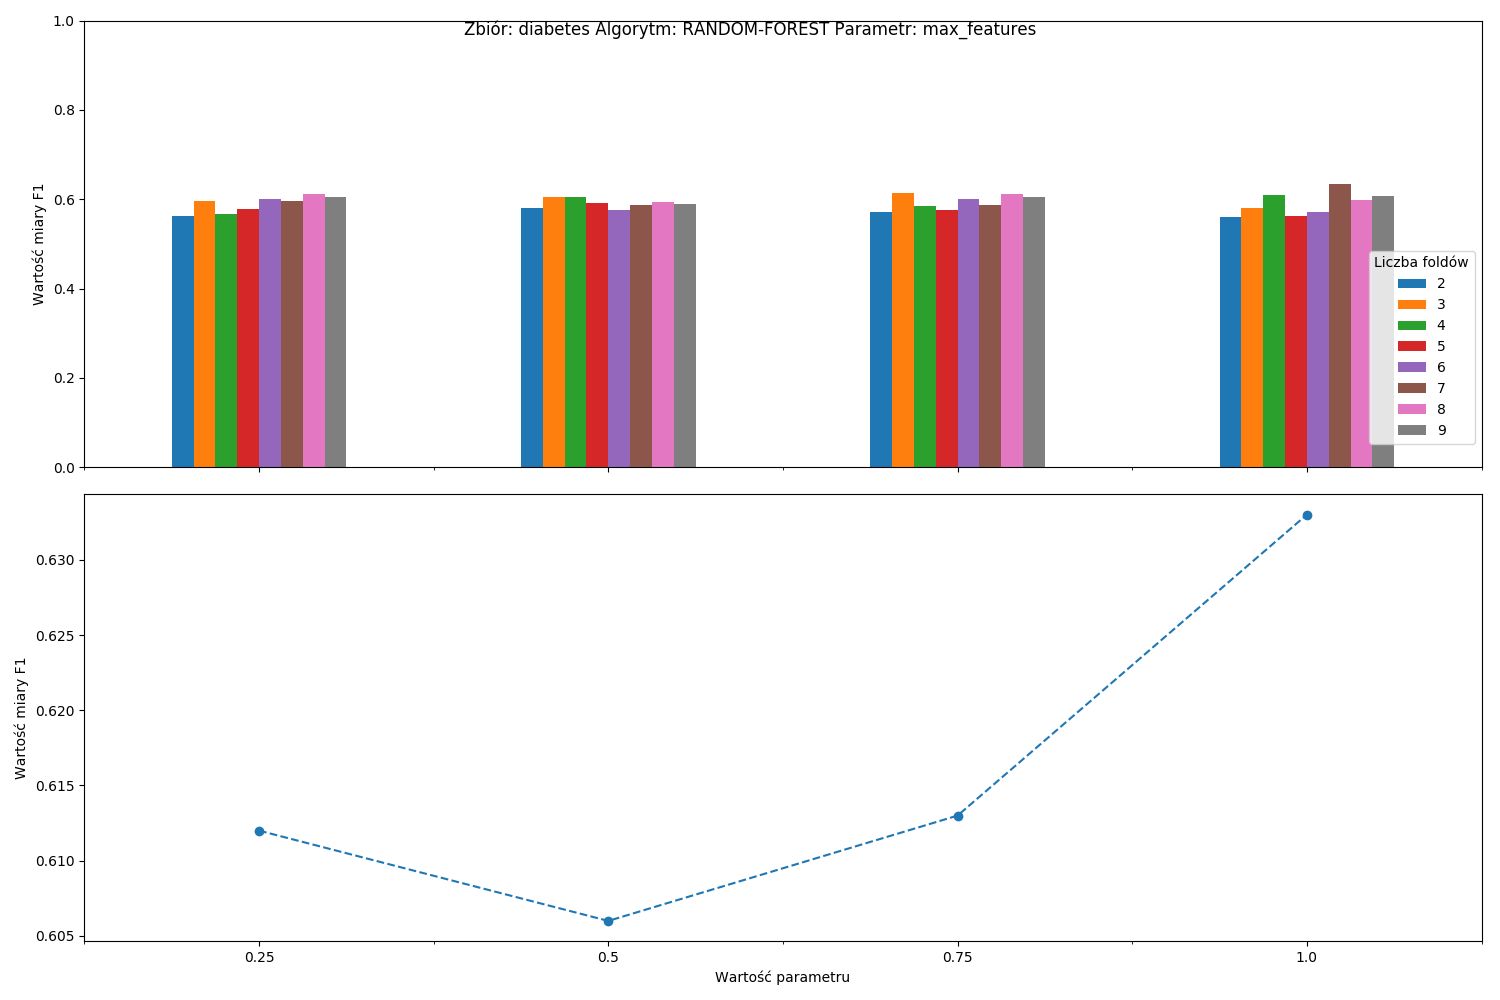
\includegraphics[width=\textwidth]{resources/plots/diabetes_random-forest_max_features.png}
    \caption{Wykres wartości miary F1 dla zbioru "Diabetes" algorytmu "Random-forest" przy ustalonym parametrze "max\_features".}
\end{figure}

\pagebreak
    \subsection{Zbiór "Glass"}
    \begin{figure}[H]
        \center
        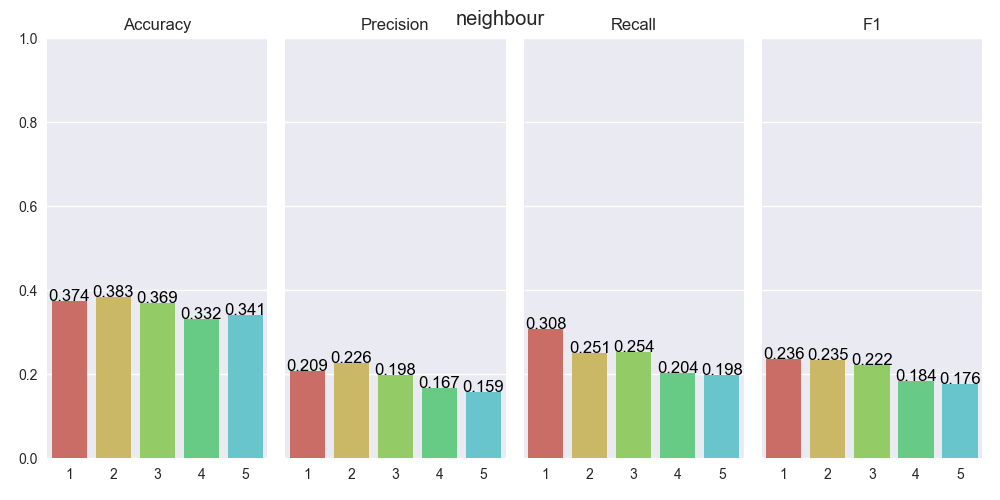
\includegraphics[width=\textwidth]{resources/plots/glass_KFold_neighbour.png}
        \caption{Wykres wartości miar dla zbioru "Glass" dla różnej liczby sąsiadów (kroswalidacja zwykła).}
    \end{figure}

    \begin{figure}[H]
        \center
        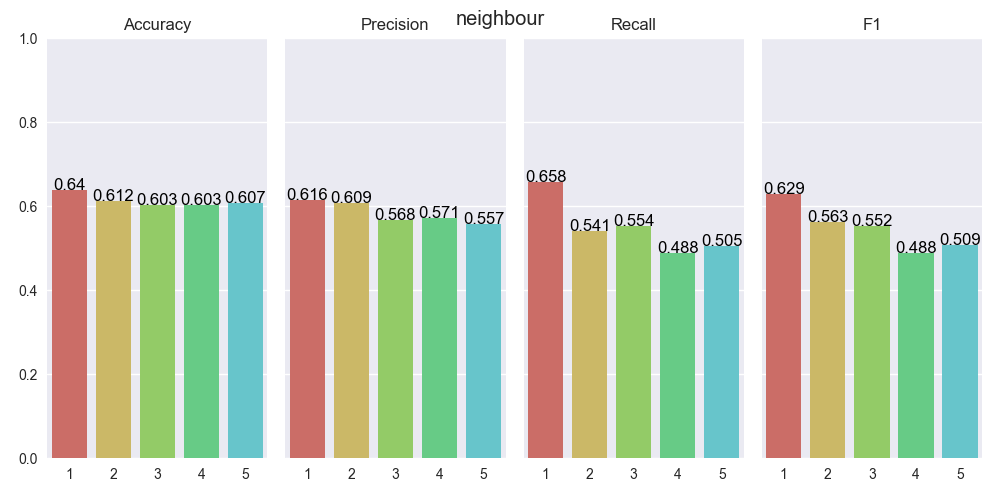
\includegraphics[width=\textwidth]{resources/plots/glass_StratifiedKFold_neighbour.png}
        \caption{Wykres wartości miar dla zbioru "Glass" dla różnej liczby sąsiadów (kroswalidacja stratyfikowana).}
    \end{figure}

    \pagebreak

    \begin{figure}[H]
        \center
        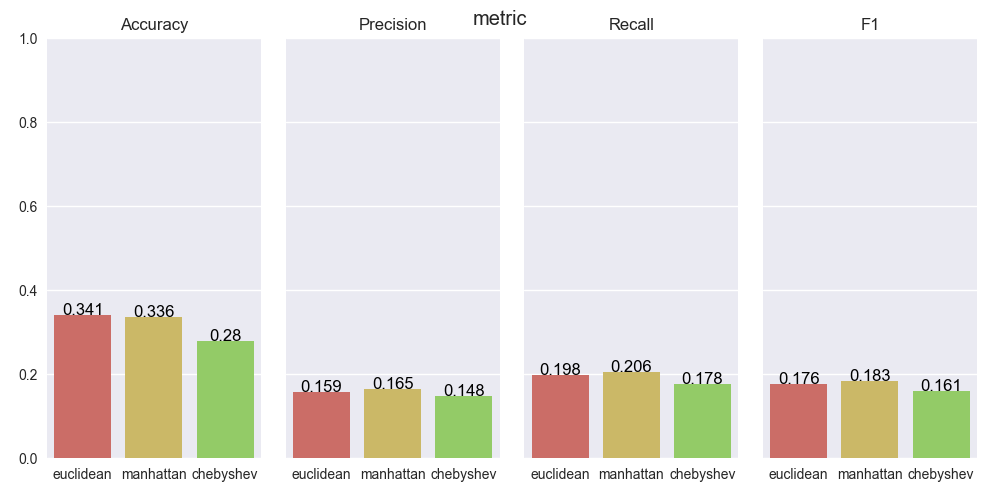
\includegraphics[width=\textwidth]{resources/plots/glass_KFold_metric.png}
        \caption{Wykres wartości miar dla zbioru "Glass" dla różnych metryk odległości (kroswalidacja zwykła).}
    \end{figure}

    \begin{figure}[H]
        \center
        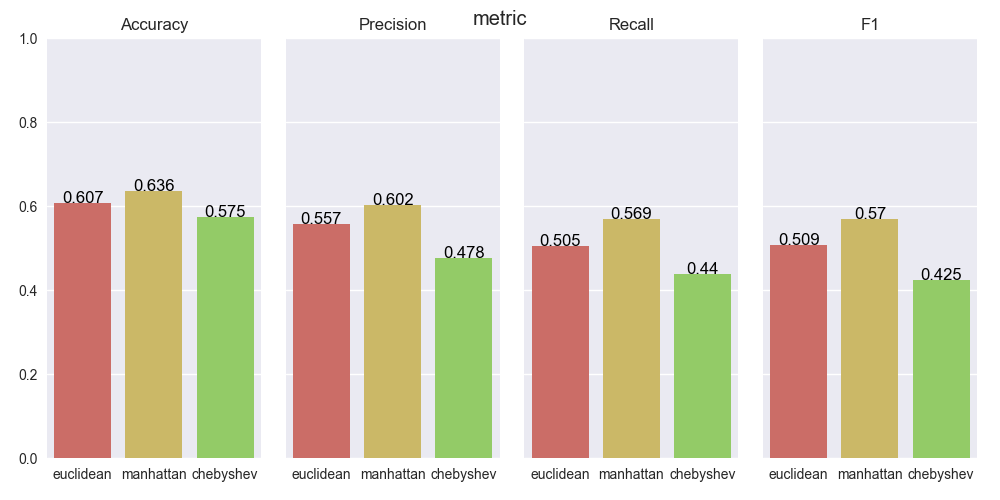
\includegraphics[width=\textwidth]{resources/plots/glass_StratifiedKFold_metric.png}
        \caption{Wykres wartości miar dla zbioru "Glass" dla różnych metryk odległości (kroswalidacja stratyfikowana).}
    \end{figure}

    \pagebreak

    \begin{figure}[H]
        \center
        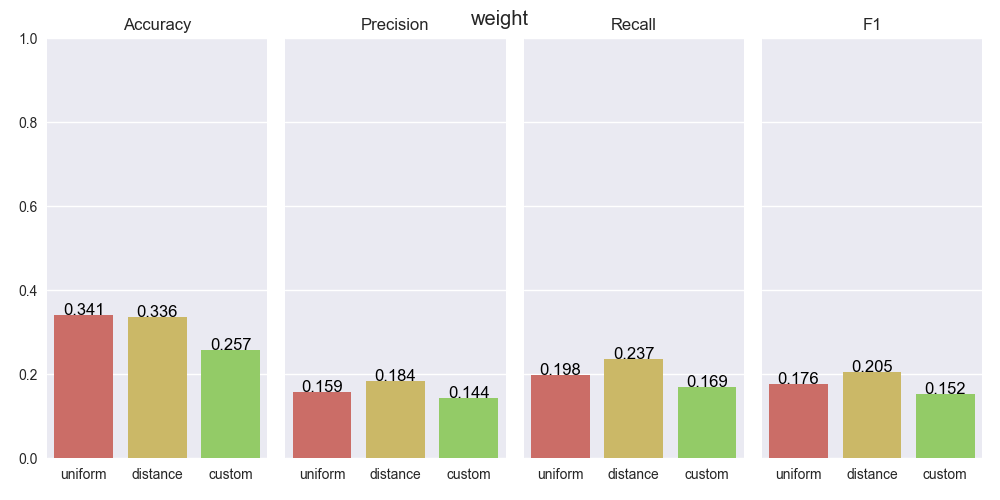
\includegraphics[width=\textwidth]{resources/plots/glass_KFold_weight.png}
        \caption{Wykres wartości miar dla zbioru "Glass" dla różnych sposobów głosowania (kroswalidacja zwykła).}
    \end{figure}

    \begin{figure}[H]
        \center
        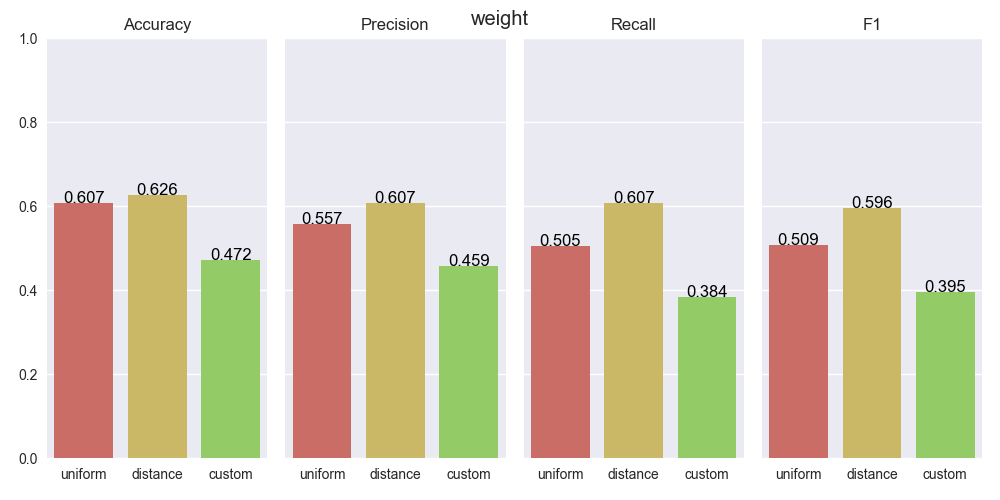
\includegraphics[width=\textwidth]{resources/plots/glass_StratifiedKFold_weight.png}
        \caption{Wykres wartości miar dla zbioru "Glass" dla różnych sposobów głosowania (kroswalidacja stratyfikowana).}
    \end{figure}

    \subsection{Zbiór "Seeds"}
    \begin{figure}[H]
        \center
        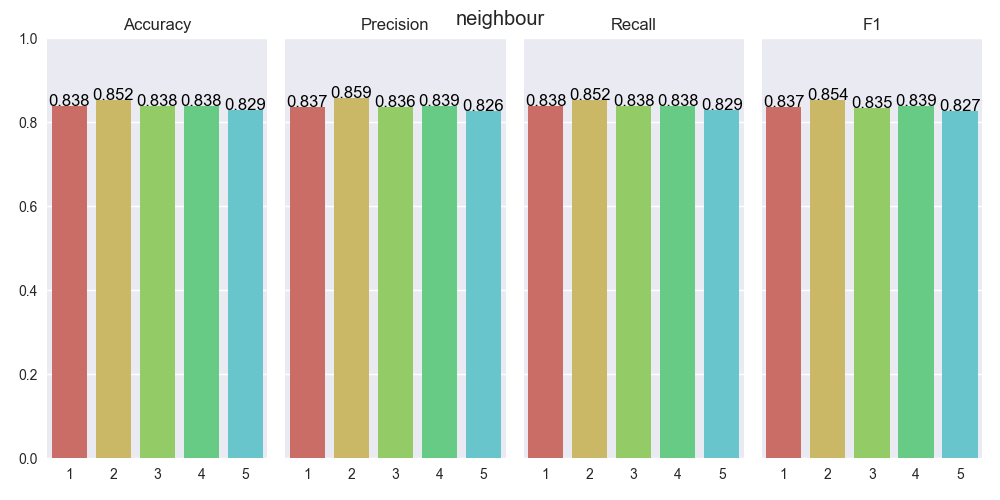
\includegraphics[width=\textwidth]{resources/plots/seeds_KFold_neighbour.png}
        \caption{Wykres wartości miar dla zbioru "Seeds" dla różnej liczby sąsiadów (kroswalidacja zwykła).}
    \end{figure}

    \begin{figure}[H]
        \center
        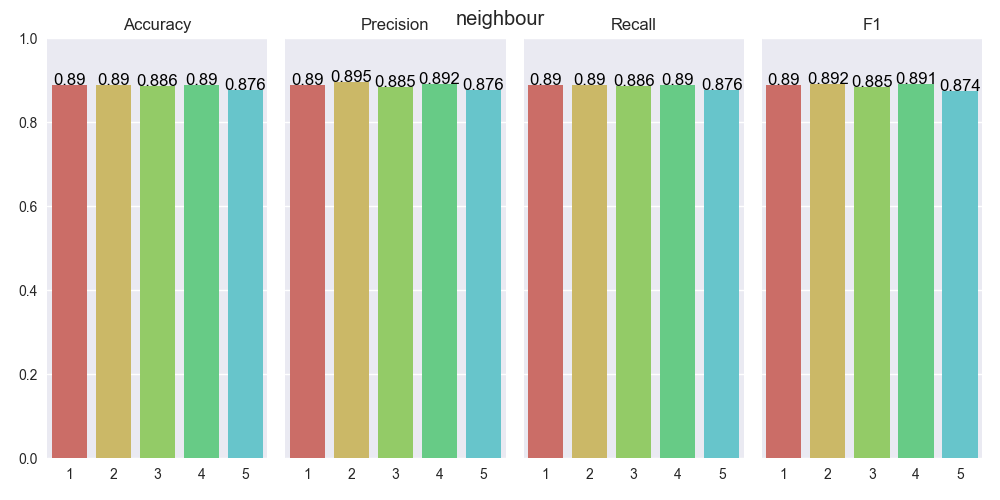
\includegraphics[width=\textwidth]{resources/plots/seeds_StratifiedKFold_neighbour.png}
        \caption{Wykres wartości miar dla zbioru "Seeds" dla różnej liczby sąsiadów (kroswalidacja stratyfikowana).}
    \end{figure}

    \pagebreak

    \begin{figure}[H]
        \center
        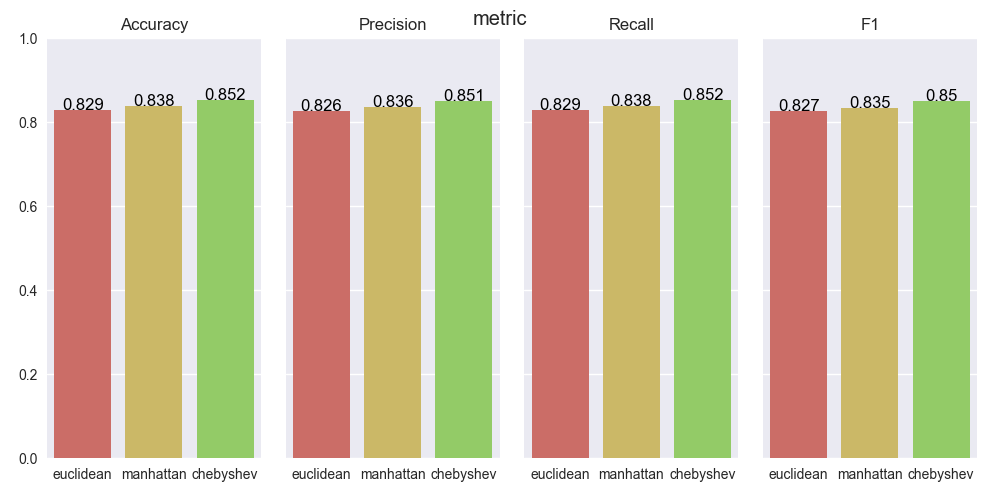
\includegraphics[width=\textwidth]{resources/plots/seeds_KFold_metric.png}
        \caption{Wykres wartości miar dla zbioru "Seeds" dla różnych metryk odległości (kroswalidacja zwykła).}
    \end{figure}

    \begin{figure}[H]
        \center
        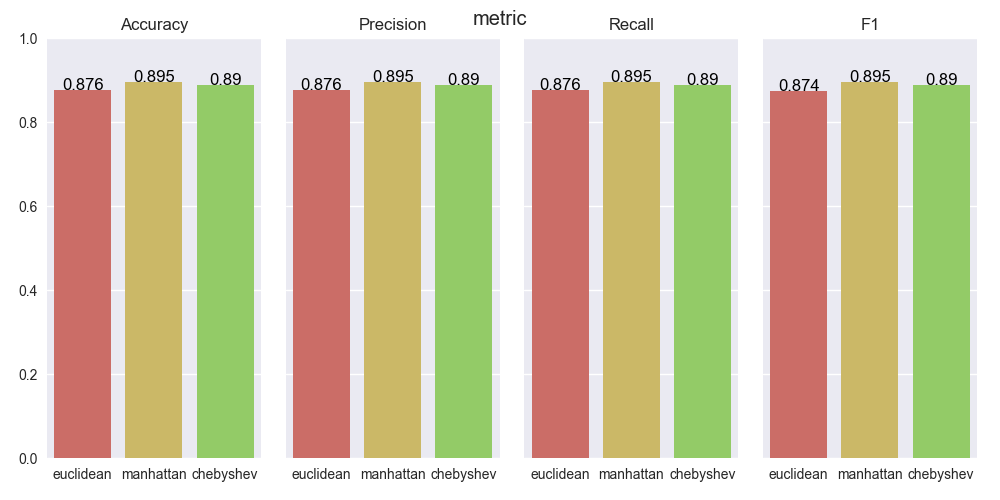
\includegraphics[width=\textwidth]{resources/plots/seeds_StratifiedKFold_metric.png}
        \caption{Wykres wartości miar dla zbioru "Seeds" dla różnych metryk odległości (kroswalidacja stratyfikowana).}
    \end{figure}

    \pagebreak

    \begin{figure}[H]
        \center
        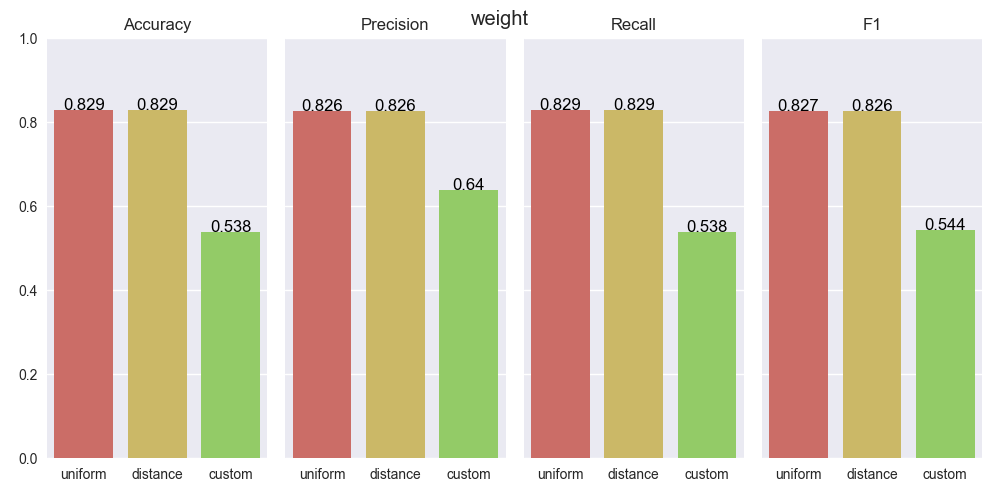
\includegraphics[width=\textwidth]{resources/plots/seeds_KFold_weight.png}
        \caption{Wykres wartości miar dla zbioru "Seeds" dla różnych sposobów głosowania (kroswalidacja zwykła).}
    \end{figure}

    \begin{figure}[H]
        \center
        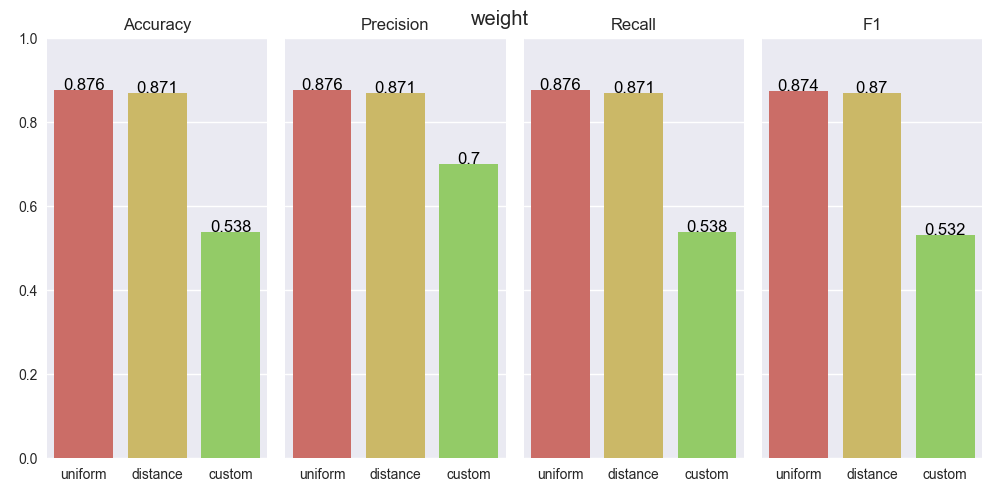
\includegraphics[width=\textwidth]{resources/plots/seeds_StratifiedKFold_weight.png}
        \caption{Wykres wartości miar dla zbioru "Seeds" dla różnych sposobów głosowania (kroswalidacja stratyfikowana).}
    \end{figure}

    \subsection{Zbiór "Wine"}
    \begin{figure}[H]
        \center
        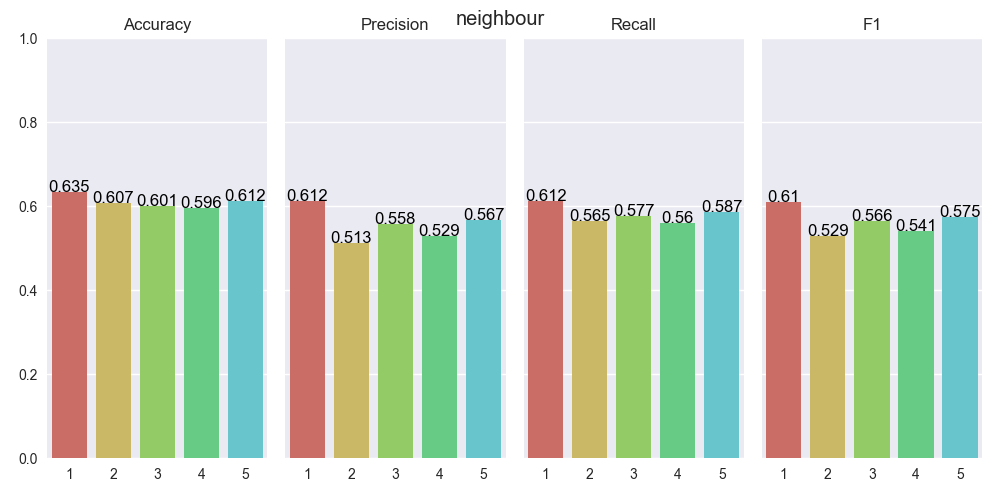
\includegraphics[width=\textwidth]{resources/plots/wine_KFold_neighbour.png}
        \caption{Wykres wartości miar dla zbioru "Wine" dla różnej liczby sąsiadów (kroswalidacja zwykła).}
    \end{figure}

    \begin{figure}[H]
        \center
        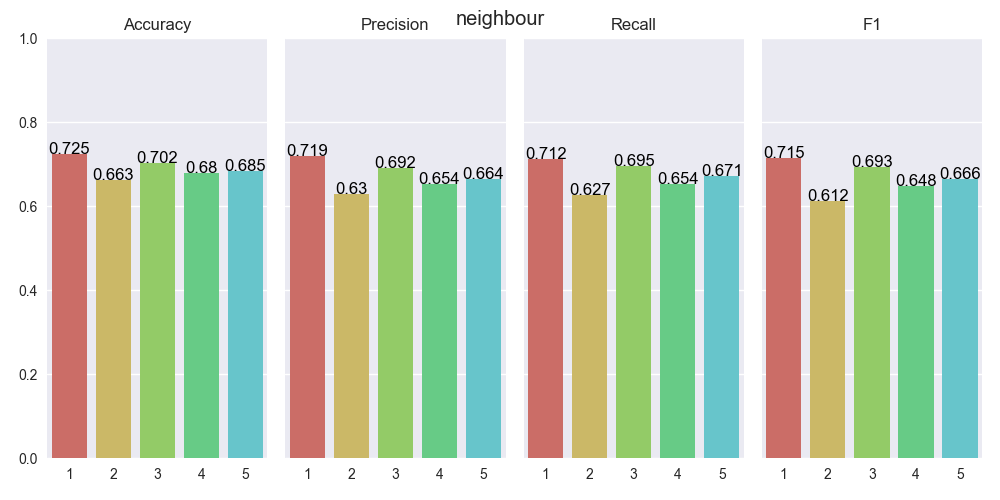
\includegraphics[width=\textwidth]{resources/plots/wine_StratifiedKFold_neighbour.png}
        \caption{Wykres wartości miar dla zbioru "Wine" dla różnej liczby sąsiadów (kroswalidacja stratyfikowana).}
    \end{figure}

    \pagebreak

    \begin{figure}[H]
        \center
        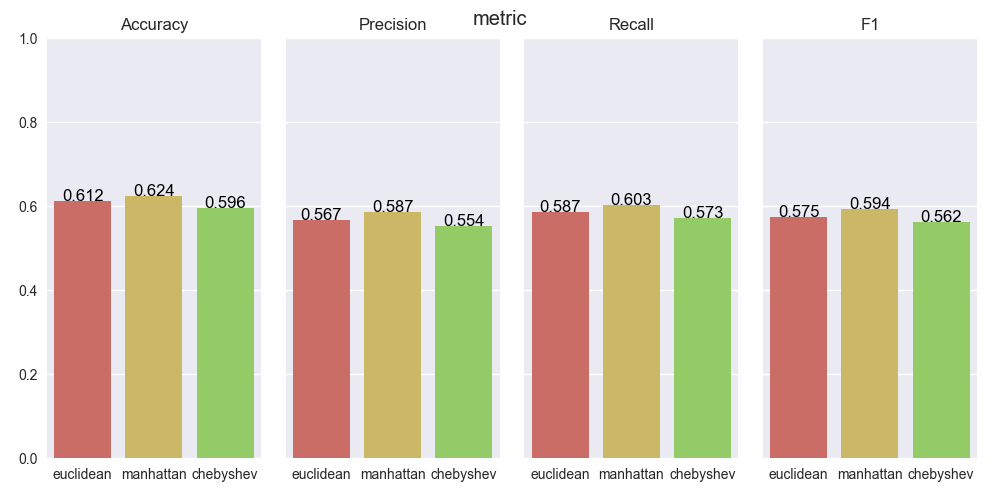
\includegraphics[width=\textwidth]{resources/plots/wine_KFold_metric.png}
        \caption{Wykres wartości miar dla zbioru "Wine" dla różnych metryk odległości (kroswalidacja zwykła).}
    \end{figure}

    \begin{figure}[H]
        \center
        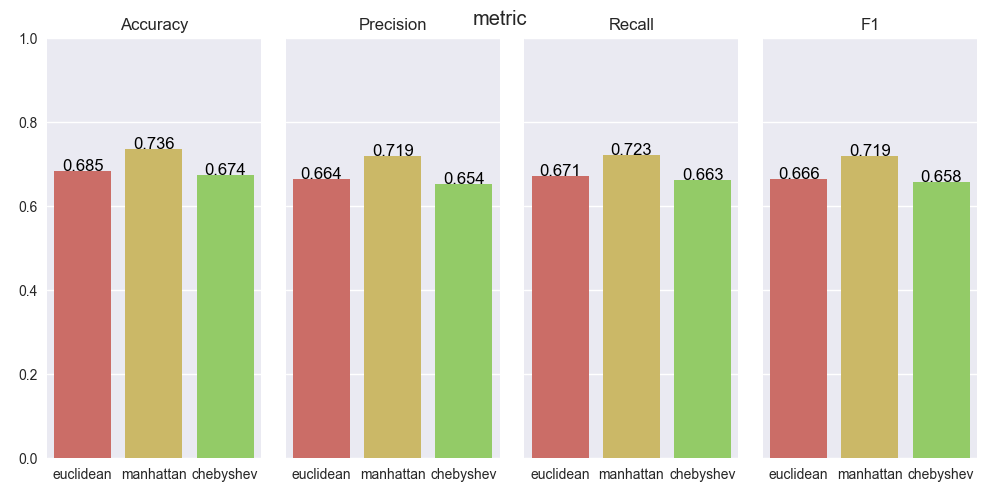
\includegraphics[width=\textwidth]{resources/plots/wine_StratifiedKFold_metric.png}
        \caption{Wykres wartości miar dla zbioru "Wine" dla różnych metryk odległości (kroswalidacja stratyfikowana).}
    \end{figure}

    \pagebreak

    \begin{figure}[H]
        \center
        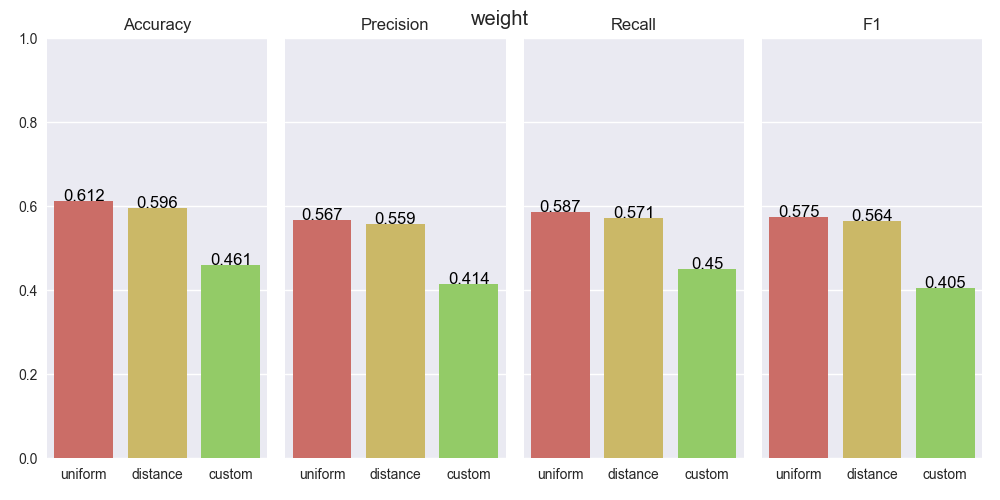
\includegraphics[width=\textwidth]{resources/plots/wine_KFold_weight.png}
        \caption{Wykres wartości miar dla zbioru "Wine" dla różnych sposobów głosowania (kroswalidacja zwykła).}
    \end{figure}

    \begin{figure}[H]
        \center
        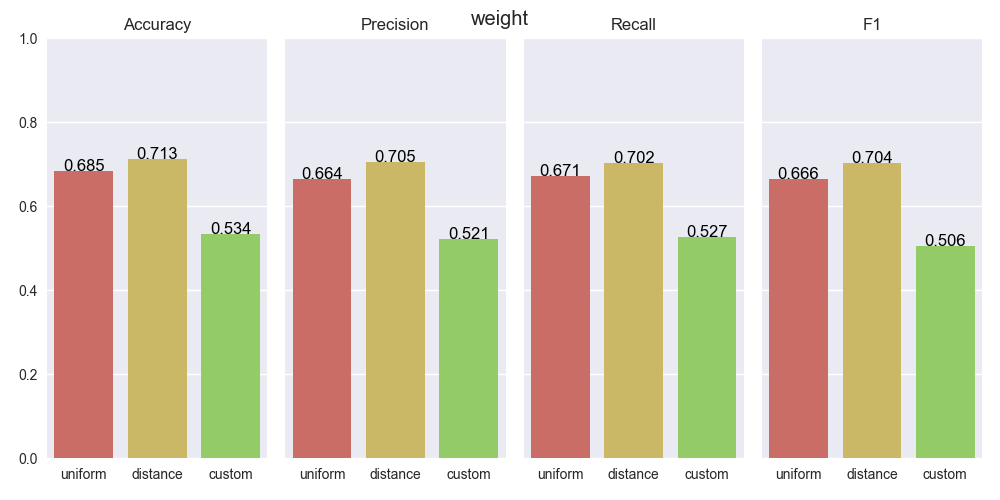
\includegraphics[width=\textwidth]{resources/plots/wine_StratifiedKFold_weight.png}
        \caption{Wykres wartości miar dla zbioru "Wine" dla różnych sposobów głosowania (kroswalidacja stratyfikowana).}
    \end{figure}

\pagebreak
\section{Porównanie klasyfikatorów}

    \begin{table}[H]
        \center
        \begin{tabular}{|c|c|c|}
            \hline
            Klasyfikator &  F1    & Komentarz \\ \hline
            C4.5         & 0.82   & CV = 6, C3 \\ \hline

            \textbf{Bagging}      & 0.64  & max\_samples = 0.5, CV = 4 (strat.) \\ \hline
            \textbf{Random-Forest}& 0.64  & n\_estimators = 10, CV = 7 (strat.) \\ \hline
            \textbf{Adaboost}     & 0.63   & learning\_rate = 0.0001, CV = 7 (strat.) \\ \hline

            Naiwny Bayes & 0.63   & CV = 6, brak dyskr. \\ \hline
            KNN          & 0.58   & CV = 5 (strat.), k = 3, euklides, głos. równ. \\ \hline
        \end{tabular}
        \caption{Najlepsze wyniki klasyfikatorów dla zbioru "Diabetes".}
    \end{table}

    \begin{table}[H]
        \center
        \begin{tabular}{|c|c|c|}
            \hline
            Klasyfikator & F1     & Komentarz \\ \hline
            C4.5         & 0.77   & CV = 8, C1 \\ \hline

            \textbf{Random-Forest}& 0.75  & criterion = entropy, CV = 8 (strat.) \\ \hline
            \textbf{Bagging}      & 0.73  & bootstrap = False, CV = 5 (strat.) \\ \hline
            \textbf{Adaboost}     & 0.72   & learning\_rate = 0.01, CV = 8 (strat.) \\ \hline

            KNN          & 0.63   & CV = 5 (strat.), k = 1, euklides, głos. równ. \\ \hline
            Naiwny Bayes & 0.61   & CV = 5, CAIM \\ \hline
        \end{tabular}
        \caption{Najlepsze wyniki klasyfikatorów dla zbioru "Glass".}
    \end{table}

    \begin{table}[H]
        \center
        \begin{tabular}{|c|c|c|}
            \hline
            Klasyfikator & F1     & Komentarz \\ \hline
            \textbf{Adaboost}     & 0.98   & learning\_rate = 0.1, CV = 7 (strat.) \\ \hline
            \textbf{Bagging}      & 0.98   & max\_samples = 1.0, CV = 5 (strat.) \\ \hline
            \textbf{Random-Forest}& 0.98  & n\_estimators = 10, CV = 7 (strat.) \\ \hline

            Naiwny Bayes & 0.97   & CV = 2, brak dyskr.\\ \hline
            C4.5         & 0.95   & CV = 7, C1 \\ \hline
            KNN          & 0.72   & CV = 5 (strat.), k = 5, manhatt., głos. równ. \\ \hline
        \end{tabular}
        \caption{Najlepsze wyniki klasyfikatorów dla zbioru "Wine".}
    \end{table}

\end{document}
